%=======================================================================
%  Growth for Whom? Airport Connectivity and the Distribution of National Income
%  Target: Transportation Research Part A: Policy and Practice (Elsevier)
%  SELF-CONTAINED: bibliography embedded via filecontents; all tables inline.
%  Upload this .tex plus the figures:
%     fig_horizon.png   fig_rf_quintile.png   fig_map_base_gacimax.png   fig_map_implied_gini.png
%  Compile: pdflatex -> bibtex -> pdflatex x2
%  Built 2026-09-18 from main_inequality_v2.tex + appendix_inequality_v2.tex (polished draft v2),
%  formatted to match the companion GACI-trade Overleaf project.
%=======================================================================
\begin{filecontents*}[overwrite]{GACI_Inequality_refs.bib}
@article{Brueckner_2003, title={Airline Traffic and Urban Economic Development}, volume={40}, ISSN={1360-063X}, DOI={10.1080/0042098032000094388}, number={8}, journal={Urban Studies}, publisher={SAGE}, author={Brueckner, Jan K.}, year={2003}, month=July, pages={1455--1469} }

@article{Allen_2014, title={Information Frictions in Trade}, volume={82}, ISSN={0012-9682}, DOI={10.3982/ecta10984}, number={6}, journal={Econometrica}, publisher={The Econometric Society}, author={Allen, Treb}, year={2014}, month=Nov, pages={2041--2083} }

@article{Feyrer_2019, title={Trade and Income---Exploiting Time Series in Geography}, volume={11}, ISSN={1945-7707}, DOI={10.1257/app.20170616}, number={4}, journal={American Economic Journal: Applied Economics}, publisher={American Economic Association}, author={Feyrer, James}, year={2019}, month=Oct, pages={1--35} }
@article{Cheung_2020,
  author = {Cheung, Tommy King-Yin and Wong, Collin Wai-Hung and Zhang, Anming},
  title = {The evolution of aviation network: Global airport connectivity index 2006--2016},
  journal = {Transportation Research Part E: Logistics and Transportation Review},
  volume = {133}, pages = {101826}, year = {2020}
}
@article{Redding_2004,
  author = {Redding, Stephen and Venables, Anthony J.},
  title = {Economic geography and international inequality},
  journal = {Journal of International Economics},
  volume = {62}, number = {1}, pages = {53--82}, year = {2004}
}
@article{Khadaroo_2008,
  author = {Khadaroo, Jameel and Seetanah, Boopen},
  title = {The role of transport infrastructure in international tourism development: A gravity model approach},
  journal = {Tourism Management},
  volume = {29}, number = {5}, pages = {831--840}, year = {2008}
}
@article{Yue_2026,
  author = {Yue, Shuai and Wang, Yixuan and Cao, Fangyu and Wang, Chunan and Jiang, Changmin and Cheung, Tommy King-Yin},
  title = {Not all runways lead to growth: Global airport connectivity and economic development},
  journal = {Transportation Research Part A: Policy and Practice},
  year = {2026},
  note = {Revised manuscript, YTRA-D-26-01594R1}
}
@article{Solt_2020,
  author = {Solt, Frederick},
  title = {Measuring income inequality across countries and over time: The Standardized World Income Inequality Database},
  journal = {Social Science Quarterly},
  volume = {101}, number = {3}, pages = {1183--1199}, year = {2020}
}
@misc{WID_2024,
  author = {{World Inequality Lab}},
  title = {World Inequality Database},
  year = {2024},
  howpublished = {\url{https://wid.world}}
}
\end{filecontents*}

\documentclass[review,3p,times,authoryear]{elsarticle}

\usepackage{lineno,hyperref}
\usepackage{amsmath,amssymb}
\usepackage{graphicx}
\usepackage{booktabs}
\usepackage{threeparttable}
\usepackage{multirow}
\usepackage{url}
\usepackage{float}

% --- Reference-list formatting (TRA / Elsevier Harvard): DOIs as https://doi.org/... links,
%     no "doi:" / "URL:" prefixes, URLs in text font (Guide for Authors sample style).
\urlstyle{same}
\providecommand{\DOIprefix}{}\renewcommand{\DOIprefix}{}
\providecommand{\URLprefix}{}\renewcommand{\URLprefix}{}
\providecommand{\doi}[1]{}\renewcommand{\doi}[1]{\href{https://doi.org/#1}{\nolinkurl{https://doi.org/#1}}}

% --- Figure/table captions: elsarticle sets captions in \footnotesize; use \small with a bold label.
\makeatletter
\long\def\@makecaption#1#2{%
  \vskip\abovecaptionskip\small
  \sbox\@tempboxa{\textbf{#1.} #2}%
  \ifdim \wd\@tempboxa >\hsize
    \textbf{#1.} #2\par
  \else
    \global \@minipagefalse
    \hb@xt@\hsize{\hfil\box\@tempboxa\hfil}%
  \fi
  \vskip\belowcaptionskip}
\makeatother
\journal{Transportation Research Part A: Policy and Practice}

\newcommand{\sym}[1]{\ensuremath{^{#1}}}

\begin{document}

\begin{frontmatter}

\title{Growth for Whom? Airport Connectivity and the Distribution of National Income}

\author[a]{Sunbin Yoo\corref{cor1}}
\ead{[email]}
\cortext[cor1]{Corresponding author.}
\author[a]{[Co-author]}
\address[a]{[Affiliation]}

\begin{abstract}
Gateway airports are associated with national income growth, but the distribution of that growth within countries has not been established. We combine the Global Airport Connectivity Index (GACI) for 1996--2023 with market and disposable income Gini coefficients from the Standardized World Income Inequality Database and pretax income shares from the World Inequality Database for 166 economies. Within-country increases in the connectivity of a country's primary hub are associated with a higher market-income Gini coefficient. The association is present in OLS with country and year fixed effects and larger in two-stage least squares that instrument connectivity with a Feyrer-type interaction between a global aviation-intensity index and baseline geographic air market access, and with a tourism-heritage instrument; the two instruments give statistically indistinguishable estimates. The market-Gini association is robust to continent by year fixed effects, to controls for baseline exposures interacted with the aviation index, and to income and inequality tercile by year fixed effects, whereas the disposable-income association is not robust to continent by year fixed effects. The response is located in the lower half of the distribution: the pretax income share of the bottom half falls, the top decile share rises by less, and the top percentile share does not respond. Connectivity raises GDP per capita, industrial employment and urbanisation, each of which is associated with lower inequality, so the residual association exceeds the total. Measured in income levels rather than shares, the same movement raises the average income of the top decile by about three times that of the bottom half, and the level estimates, unlike the ratio between the two, survive neither continent by year fixed effects nor the second instrument. Holding total national connectivity fixed, a more concentrated airport network is associated with higher inequality. Long-difference and Open Skies liberalisation designs do not move connectivity, so the evidence identifies within-country co-movement rather than the response to a discrete shock. The association is strongest in Asia and in the period after 2010.
\end{abstract}

\begin{keyword}
Air connectivity \sep income inequality \sep Gini coefficient \sep
shift-share instrument \sep hub concentration \sep redistribution
\end{keyword}

\end{frontmatter}

\linenumbers

\section{Introduction}
\label{sec:intro}
Whether air connectivity raises national income has been established in the accessibility literature; whether the resulting income is shared has not. Recent global evidence links the connectivity of a country's most connected airport to GDP per capita, inbound tourism and service exports, with the largest GDP association in the lowest development quartile \citep{Yue_2026}. National aggregates cannot show who receives these gains. A gateway hub concentrates high-skill business services, tourism employment and land rents in one metropolitan area, while the traffic it carries originates throughout the country. The distributional consequences of this concentration are the subject of this paper.

We ask whether hub connectivity makes national income more unequal. Connectivity is measured with the Global Airport Connectivity Index (GACI), which combines degree, eigenvector, closeness and flow-betweenness centrality with regional importance for 5,428 airports over 1996--2024 \citep{Cheung_2020}. Inequality is measured with the market and disposable income Gini coefficients of the Standardized World Income Inequality Database (SWIID) and with the pretax and post-tax income shares of the World Inequality Database (WID). The estimation sample covers 166 economies and 3,735 country-years.

Three features of the design are central. First, market and disposable inequality are treated separately, so that the response can be decomposed into a market component and a redistribution component. Second, the Gini is complemented with the income shares of the bottom half, the top decile and the top percentile, so that the location of the response along the distribution is observed rather than inferred. Third, two instruments that exploit different sources of variation are used, a Feyrer-type interaction between a global aviation-intensity index and each country's baseline geographic air market access \citep{Feyrer_2019} and a tourism-heritage interaction between world tourist arrivals and a country's fixed endowment of natural World Heritage sites. Because both instruments share the shift-share structure, whose validity depends on baseline exposures being unrelated to differential inequality trends, an extensive set of exposure-trend diagnostics is reported.

The paper makes three contributions. First, it provides the first global panel estimates of the association between airport connectivity and the within-country distribution of income. Second, it locates the response along the distribution and separates the market response from redistribution. Third, it shows that the composition of a national airport network is associated with the distribution of income conditional on the total amount of connectivity, which bears on the policy choice between hub concentration and distributed airport investment.

\section{Hypothesis development}
\label{sec:framework}
Four channels connect the connectivity of a national gateway to the distribution of income, and they do not all operate in the same direction, which is why the question is empirical.

The first channel is skill-biased demand. Hub connectivity lowers the cost of face-to-face interaction and therefore raises the demand for tradable business services, finance and professional occupations, which are concentrated among high earners \citep{Allen_2014,Brueckner_2003}. If this channel dominates, the top of the distribution gains. The second channel is tourism employment. Connectivity raises inbound tourism, whose direct employment is concentrated in accommodation and food services and is low-wage \citep{Khadaroo_2008}. If this channel dominates, the bottom of the distribution gains and inequality falls. The third channel is spatial concentration. A gateway city captures the location rents and agglomeration gains of connectivity, while the rest of the country supplies migrants and demand; the resulting interregional gap appears in national personal inequality \citep{Redding_2004}. The fourth channel is redistribution. Market inequality may rise while disposable inequality rises by less if governments redistribute part of the gains.

\begin{quote}
\textbf{Hypothesis 1 (Distribution).} Higher hub connectivity increases the market-income Gini coefficient. The disposable-income response is smaller than the market-income response.
\end{quote}
\begin{quote}
\textbf{Hypothesis 2 (Location).} The response is located at the tails: the pretax income share of the top decile rises and the share of the bottom half falls.
\end{quote}
\begin{quote}
\textbf{Hypothesis 3 (Concentration).} Conditional on total national connectivity, a network in which connectivity is concentrated in a single gateway is associated with higher inequality than a distributed network.
\end{quote}
\begin{quote}
\textbf{Hypothesis 4 (Mechanisms).} The association operates net of the income growth, structural transformation and urbanisation that connectivity induces; these induced changes are themselves associated with lower inequality, so that the residual association exceeds the total.
\end{quote}

\section{Data}
\label{sec:data}
The panel combines the airport-year GACI data of the companion papers with three inequality sources. Connectivity is aggregated to the country-year in three ways: the maximum across the country's airports (hub connectivity, $\mathrm{GACI}_{max}$), the seat-capacity-weighted mean (hub quality, $\mathrm{GACI}_{cwm}$) and the sum across airports (total connectivity, $\mathrm{GACI}_{sum}$). Two concentration measures summarise the composition of the network: the share of the top airport in the national sum and the Herfindahl index of airport shares.

Inequality is measured in three ways. The SWIID (version 9) provides market-income and disposable-income Gini coefficients for 199 economies with model-based standard errors; we use the point estimates and report country-clustered inference throughout \citep{Solt_2020}. The WID provides pretax and post-tax national income shares for the bottom 50 percent, the middle 40 percent, the top 10 percent and the top 1 percent of equal-split adults, together with a Gini derived from the same distributions \citep{WID_2024}. The World Bank Poverty and Inequality Platform provides survey-based Gini coefficients and decile shares for survey years only and serves as an independent check. Controls and mechanism variables (population, GDP per capita, sectoral employment shares, urbanisation, urban primacy, unemployment, trade, FDI, tax revenue and tertiary enrolment) come from the World Development Indicators.

The estimation sample is the intersection of the connectivity panel with the SWIID: 166 economies and 3,735 country-years over 1996--2023. Table~\ref{tab:sumstat} reports summary statistics. Two features of the data matter for what follows. First, inequality is slow moving: the within-country standard deviation of the market Gini is 1.7 points against a cross-sectional standard deviation of 6.4. Second, hub connectivity also varies mainly across countries: the within standard deviation of $\ln\mathrm{GACI}_{max}$ is 0.16 against 0.61 overall. Both features limit the information available in short differences, to which we return in Section~\ref{sec:horizon}.

\begin{table}[H]\centering\caption{Summary statistics, estimation sample (166 economies, 1996--2023).}\label{tab:sumstat}
\begin{threeparttable}\small\begin{tabular}{lrrrrrr}
\toprule
Variable & N & Mean & SD & Within SD & Min & Max \\
\midrule
Market-income Gini (SWIID) & 3,737 & 45.594 & 6.413 & 1.672 & 31.200 & 72.400 \\
Disposable-income Gini (SWIID) & 3,737 & 38.363 & 8.193 & 1.678 & 22.100 & 65.800 \\
Top 10\% pretax income share (WID) & 3,716 & 0.453 & 0.093 & 0.025 & 0.255 & 0.687 \\
Bottom 50\% pretax income share (WID) & 3,716 & 0.150 & 0.047 & 0.012 & 0.051 & 0.279 \\
Hub connectivity, GACI max & 3,737 & 1.319 & 0.612 & 0.157 & 0.534 & 3.626 \\
Hub quality, GACI cwm & 3,737 & 1.124 & 0.416 & 0.115 & 0.534 & 3.014 \\
Total connectivity, GACI sum & 3,737 & 16.589 & 46.228 & 6.274 & 0.545 & 510.036 \\
Share of top airport in national GACI & 3,737 & 0.366 & 0.329 & 0.105 & 0.006 & 1.000 \\
Airports per country & 3,737 & 22.272 & 57.942 & 6.996 & 1.000 & 614.000 \\
Feyrer instrument & 3,737 & 4.606 & 4.227 & 4.104 & 0.000 & 14.667 \\
Tourism-heritage instrument & 3,737 & 0.475 & 0.478 & 0.276 & 0.000 & 2.944 \\
ln population & 3,737 & 16.095 & 1.805 & 0.125 & 9.778 & 21.078 \\
ln GDP per capita & 3,737 & 8.587 & 1.446 & 0.222 & 5.426 & 11.630 \\
\bottomrule
\end{tabular}
\begin{tablenotes}\footnotesize\item Within SD is the standard deviation after removing country means. Gini coefficients in points; income shares as fractions.\end{tablenotes}\end{threeparttable}\end{table}

Figure~\ref{fig:map_base} maps hub connectivity in 2023. The gateway economies of North America, Western Europe, the Gulf and East Asia occupy the top of the distribution and most of sub-Saharan Africa and Central Asia the bottom; the cross-sectional range of $\ln\mathrm{GACI}_{max}$ is $-0.55$ to $1.18$ against a within-country standard deviation of $0.16$.

\begin{figure}[H]\centering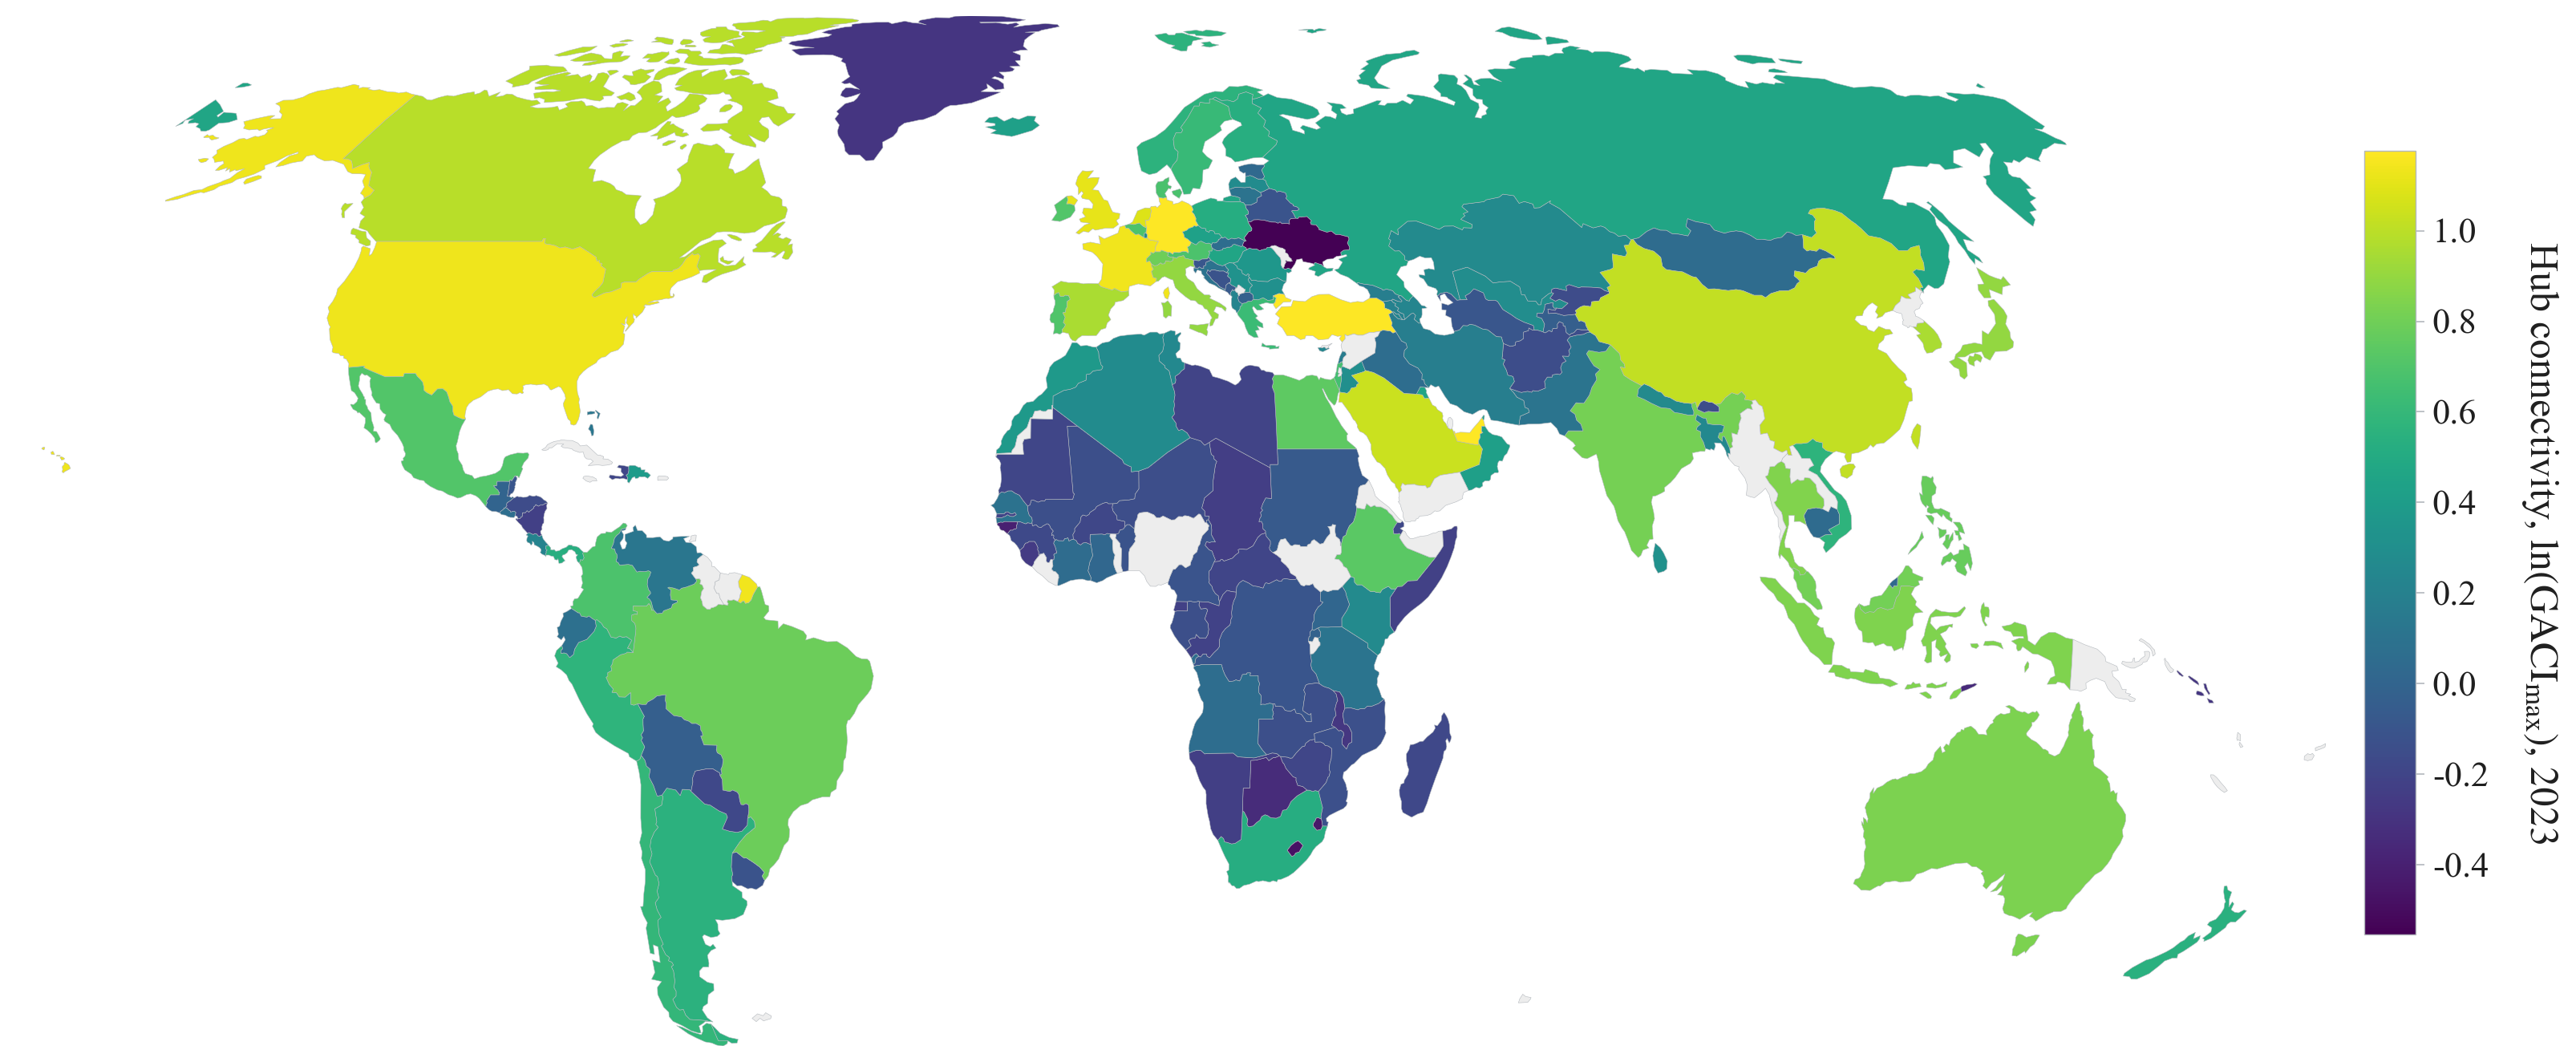
\includegraphics[width=\linewidth]{fig_map_base_gacimax.png}
\caption{Hub connectivity, $\ln\mathrm{GACI}_{max}$, 2023. Grey denotes economies outside the estimation sample.}\label{fig:map_base}\end{figure}

\section{Empirical strategy}
\label{sec:strategy}
The baseline specification relates within-country changes in inequality to within-country changes in connectivity:
\begin{equation}
\ln G_{ct} = \beta \ln \mathrm{GACI}_{ct} + \gamma \ln \mathrm{Pop}_{ct} + \mu_c + \lambda_t + \varepsilon_{ct},
\label{eq:base}
\end{equation}
where $G_{ct}$ is the Gini coefficient or an income share of country $c$ in year $t$, and $\mu_c$ and $\lambda_t$ are country and year fixed effects. Following the companion papers, the baseline controls only for population; GDP per capita, trade and the sectoral structure are outcomes of connectivity and enter as candidate mechanisms rather than as controls. Standard errors are heteroskedasticity-robust in the main tables, with country-clustered standard errors reported in brackets and used for the two-stage least squares (2SLS) inference in the text.

Connectivity is not assigned at random. Route development follows expected demand, and the policy reforms that attract airlines may also change the distribution of income. We therefore instrument $\ln\mathrm{GACI}_{ct}$ with the Feyrer interaction $Z^{F}_{ct} = a_t \times \ln\mathrm{MA}^{air}_{c,1996}$, where $a_t$ is a global aviation-intensity index normalised to $[0,1]$ and $\mathrm{MA}^{air}_{c,1996}$ is the population-weighted great-circle market access of the country's airports in the base year \citep{Feyrer_2019}. The identifying assumption is that, conditional on the fixed effects, countries whose geography placed them to benefit more from the global expansion of aviation did not experience differential inequality trends for other reasons. The tourism-heritage instrument $Z^{T}_{ct}$ interacts world international tourist arrivals with the country's fixed endowment of natural and mixed World Heritage sites and identifies connectivity growth on the leisure margin. The two instruments differ in the exposure they use, so agreement between them is informative, and the Hansen $J$ test of over-identification is reported.

Both instruments are shift-share instruments with a single global shifter. Their validity therefore rests on the exposure variable, which we probe in four ways in Section~\ref{sec:diag}: continent by year fixed effects, controls for other baseline exposures (income, inequality, land area, latitude, sea market access) interacted with the same aviation index, income and inequality tercile by year fixed effects, and first stages estimated separately by continent.

\section{Main results}
\label{sec:results}
We begin by asking whether hub connectivity is associated with the level of inequality within countries. This is the first-order question for the distributional reading of connectivity: if the market Gini does not move with the primary hub, the channels in Section~\ref{sec:framework} cancel in the aggregate. Table~\ref{tab:main} reports, for each connectivity measure, the OLS estimate, the first stage of each instrument and the 2SLS estimates for the market and disposable Gini coefficients. All specifications include country and year fixed effects and log population; first-stage statistics are reported within the table.

Panel A uses hub connectivity, the headline measure. In OLS, a one-percent increase in hub connectivity is associated with a $0.061$ percent increase in the market Gini. The 2SLS estimate is $0.495$ with the Feyrer instrument and $0.468$ with the tourism instrument, and the two instruments therefore agree on sign and magnitude; the Hansen $J$ test does not reject their joint validity for the market Gini ($p=0.88$, Table~\ref{tab:robust}). For example, a coefficient of $0.495$ means that a 10 percent increase in hub connectivity is associated with a 5 percent increase in the market Gini, or about 2.3 points at the sample mean of 45.6. The disposable Gini responds by a similar amount in OLS ($0.050$) and by more in 2SLS ($0.651$ with the Feyrer instrument, $0.391$ with the tourism instrument). The first part of Hypothesis~1 is supported; the second part, that redistribution attenuates the response, is not, since the disposable response is not smaller than the market response.

Panel B uses hub quality and Panel C total connectivity. The pattern of signs and significance is unchanged. The sum measure has the smallest coefficients because it scales with the number of airports, and the capacity-weighted mean has the largest, consistent with connectivity concentrated at large airports being the relevant margin. The three measures are on different scales; what carries across them is the common pattern of a positive OLS estimate, a larger 2SLS estimate, and agreement between the two instruments. Table~\ref{tab:a_levels} reports the same specifications with the Gini in points, and Table~\ref{tab:a_absred} reports absolute redistribution as an outcome.

The 2SLS estimates are about eight times the OLS estimates. Three explanations are consistent with the data. First, measurement error in the aggregated index attenuates OLS. Second, the instruments identify the response of countries whose connectivity growth was driven by global aviation expansion and geography, which may be the countries in which connectivity growth was least accompanied by compensating policy. Third, the instruments may partly capture differential trends, which Section~\ref{sec:diag} examines. We report both estimates throughout and treat the OLS estimate as a lower bound and the 2SLS estimate as an upper bound when quantifying the association.

\begin{table}[H]\centering\caption{Main results: OLS, first stage, and 2SLS, by connectivity measure.}\label{tab:main}
\begin{threeparttable}\small\begin{tabular}{lcc}
\toprule
 & Market-income Gini & Disposable-income Gini \\
 & $\ln G^{mkt}$ & $\ln G^{disp}$ \\
\midrule
\multicolumn{3}{l}{\emph{Panel A. Hub connectivity, $\ln\mathrm{GACI}_{max}$ (headline)}}\\
First stage, Feyrer instrument & \multicolumn{2}{l}{0.146\sym{***}\ \ (0.015),\ \ KP $F=98.5$} \\
First stage, Tourism-heritage instrument & \multicolumn{2}{l}{0.038\sym{***}\ \ (0.010),\ \ KP $F=13.6$} \\
OLS & 0.061\sym{***} (0.008) & 0.050\sym{***} (0.009) \\
2SLS, Feyrer IV & 0.495\sym{***} (0.062) & 0.651\sym{***} (0.077) \\
 & [0.194]\sym{**} & [0.241]\sym{***} \\
2SLS, tourism IV & 0.468\sym{***} (0.165) & 0.391\sym{***} (0.151) \\
 & [0.260]\sym{*} & [0.284] \\
\addlinespace
\multicolumn{3}{l}{\emph{Panel B. Hub quality, $\ln\mathrm{GACI}_{cwm}$}}\\
First stage, Feyrer instrument & \multicolumn{2}{l}{0.122\sym{***}\ \ (0.013),\ \ KP $F=83.2$} \\
First stage, Tourism-heritage instrument & \multicolumn{2}{l}{0.024\sym{***}\ \ (0.009),\ \ KP $F=6.9$} \\
OLS & 0.079\sym{***} (0.009) & 0.060\sym{***} (0.010) \\
2SLS, Feyrer IV & 0.595\sym{***} (0.076) & 0.783\sym{***} (0.096) \\
 & [0.240]\sym{**} & [0.302]\sym{***} \\
2SLS, tourism IV & 0.726\sym{**} (0.313) & 0.607\sym{**} (0.283) \\
 & [0.547] & [0.530] \\
\addlinespace
\multicolumn{3}{l}{\emph{Panel C. Total connectivity, $\ln\mathrm{GACI}_{sum}$}}\\
First stage, Feyrer instrument & \multicolumn{2}{l}{0.364\sym{***}\ \ (0.034),\ \ KP $F=113.4$} \\
First stage, Tourism-heritage instrument & \multicolumn{2}{l}{0.068\sym{***}\ \ (0.023),\ \ KP $F=9.0$} \\
OLS & 0.008\sym{***} (0.002) & 0.009\sym{***} (0.003) \\
2SLS, Feyrer IV & 0.199\sym{***} (0.026) & 0.262\sym{***} (0.031) \\
 & [0.077]\sym{***} & [0.090]\sym{***} \\
2SLS, tourism IV & 0.260\sym{***} (0.099) & 0.217\sym{**} (0.093) \\
 & [0.191] & [0.187] \\
\addlinespace
\midrule
Country, Year FE & Yes & Yes \\
Observations & 3,735 & 3,735 \\
\bottomrule
\end{tabular}
\begin{tablenotes}\footnotesize\item Robust SE in parentheses; country-clustered SE in brackets with the corresponding significance level. The first-stage rows regress the connectivity measure on the instrument with population and two-way fixed effects; KP $F$ is the Kleibergen--Paap statistic with robust errors. \sym{*}~$p<0.10$, \sym{**}~$p<0.05$, \sym{***}~$p<0.01$.\end{tablenotes}\end{threeparttable}\end{table}

\subsection{Growth and its incidence}
\label{sec:growth}
Does hub connectivity also move average income, and if so, who receives the increase? This matters for reading Table~\ref{tab:main}: a rising Gini that accompanies broad income growth is a different object from a rising Gini in which the bottom half stands still. Table~\ref{tab:growth} reports the specifications of Table~\ref{tab:main} with growth outcomes, and Table~\ref{tab:growth_decomp} separates the response of each group's average income into a level term that both groups share and a share term that they do not.

Average income moves with connectivity, and by more than any distribution estimate in this paper. In OLS a one-percent increase in hub connectivity accompanies a $0.75$ percent increase in GDP per capita, and in 2SLS with the Feyrer instrument the elasticity is $1.29$. The World Inequality Database measure of average pretax income per adult, which is built from national accounts rather than from the World Development Indicators, gives $0.67$ and $1.22$ in the same specifications, so the two income sources agree on the sign and on the order of magnitude.

The increase is not shared evenly. Under the Feyrer instrument the average income of the top decile rises by $1.44$ percent per percent of connectivity, the average income of the bottom half by $0.45$ percent, and the ratio between the two by $1.00$ percent. Table~\ref{tab:growth_decomp} shows where the difference arises. Both groups carry the same level term of $1.22$. The top decile adds a share gain of $0.22$ and the bottom half subtracts a share loss of $0.77$, which is the estimate already reported in Table~\ref{tab:tails}. The bottom half therefore retains about one third of the average gain. Consider an economy whose hub connectivity rises by ten percent. Average income rises by about twelve percent, the average income of the top decile by about fourteen percent and that of the bottom half by about four percent, while the market Gini rises by about five percent of its own value, which is $2.3$ points at the sample mean of $45.6$. Growth and the rise in the Gini are two readings of one movement rather than two separate findings.

The growth estimates are less robust than the distribution estimates, and three results set the limit. First, the tourism-heritage instrument, which reproduces the market-Gini estimate of the Feyrer instrument ($0.47$ against $0.50$), gives $-0.13$ for GDP per capita and cannot be distinguished from zero; with both instruments entered together the Hansen test rejects for GDP per capita ($p=0.002$), for average income ($p<0.001$) and for the top decile ($p=0.004$), but not for the top-to-bottom ratio ($p=0.33$). Second, under continent by year fixed effects the level estimates turn negative, $-1.07$ for GDP per capita and $-1.68$ for the bottom half, while the ratio remains positive at $1.21$ and significant (Table~\ref{tab:a_growth_diag}). Third, in long differences the instrument is uninformative for growth as it is for inequality, with a first-stage $F$ below $3$ in every window (Table~\ref{tab:a_growth_ld}), and the leads are as large as the lags (Table~\ref{tab:a_growth_hzn}). What survives these checks is the incidence rather than the level, so we treat the level estimates as descriptive and the gap estimates as the result.

One feature of the construction separates the two halves of Table~\ref{tab:growth_decomp}. The Gini coefficients and the income shares are distribution statistics and do not use national income in their construction, so their co-movement with GDP per capita is an estimate rather than an identity. The group average incomes in the last three columns of Table~\ref{tab:growth} do share a national-accounts level term by construction, and that term is what row 1 of Table~\ref{tab:growth_decomp} isolates and the ratio removes.

\begin{table}[H]\centering\caption{Growth outcomes: GDP per capita and group average incomes.}\label{tab:growth}
\begin{threeparttable}\small\begin{tabular}{lccccc}
\toprule
 & GDP per capita & Average income & Top 10\% average & Bottom 50\% average & Top/bottom gap \\
 & $\ln y$ & $\ln \bar{y}$ & $\ln \bar{y}^{t10}$ & $\ln \bar{y}^{b50}$ & $\ln(\bar{y}^{t10}/\bar{y}^{b50})$ \\
\midrule
\multicolumn{6}{l}{\emph{Panel A. Hub connectivity, $\ln\mathrm{GACI}_{max}$ (headline)}}\\
OLS & 0.747\sym{***} (0.042) & 0.668\sym{***} (0.043) & 0.747\sym{***} (0.042) & 0.586\sym{***} (0.051) & 0.161\sym{***} (0.034) \\
2SLS, Feyrer IV & 1.294\sym{***} (0.152) & 1.219\sym{***} (0.173) & 1.443\sym{***} (0.184) & 0.445\sym{**} (0.200) & 0.998\sym{***} (0.189) \\
 & [0.428]\sym{***} & [0.491]\sym{**} & [0.513]\sym{***} & [0.593] & [0.588]\sym{*} \\
2SLS, tourism IV & -0.133 (0.559) & -0.394 (0.573) & -0.013 (0.557) & -0.506 (0.622) & 0.493 (0.414) \\
 & [1.127] & [1.142] & [1.120] & [1.268] & [0.975] \\
First-stage KP $F$ (Feyrer; tourism) & 98; 14 & 97; 13 & 97; 13 & 97; 13 & 97; 13 \\
\addlinespace
\multicolumn{6}{l}{\emph{Panel B. Hub quality, $\ln\mathrm{GACI}_{cwm}$}}\\
OLS & 0.775\sym{***} (0.043) & 0.708\sym{***} (0.044) & 0.774\sym{***} (0.046) & 0.656\sym{***} (0.050) & 0.118\sym{***} (0.037) \\
2SLS, Feyrer IV & 1.556\sym{***} (0.194) & 1.462\sym{***} (0.214) & 1.731\sym{***} (0.229) & 0.533\sym{**} (0.241) & 1.197\sym{***} (0.231) \\
 & [0.548]\sym{***} & [0.611]\sym{**} & [0.633]\sym{***} & [0.715] & [0.709]\sym{*} \\
2SLS, tourism IV & -0.206 (0.882) & -0.612 (0.932) & -0.019 (0.866) & -0.785 (1.025) & 0.766 (0.682) \\
 & [1.748] & [1.791] & [1.738] & [2.027] & [1.603] \\
First-stage KP $F$ (Feyrer; tourism) & 83; 7 & 83; 7 & 83; 7 & 83; 7 & 83; 7 \\
\addlinespace
\multicolumn{6}{l}{\emph{Panel C. Total connectivity, $\ln\mathrm{GACI}_{sum}$}}\\
OLS & 0.185\sym{***} (0.012) & 0.172\sym{***} (0.012) & 0.178\sym{***} (0.013) & 0.166\sym{***} (0.013) & 0.013 (0.010) \\
2SLS, Feyrer IV & 0.520\sym{***} (0.067) & 0.497\sym{***} (0.076) & 0.589\sym{***} (0.082) & 0.181\sym{**} (0.084) & 0.407\sym{***} (0.075) \\
 & [0.173]\sym{***} & [0.200]\sym{**} & [0.213]\sym{***} & [0.246] & [0.233]\sym{*} \\
2SLS, tourism IV & -0.074 (0.312) & -0.223 (0.331) & -0.007 (0.315) & -0.286 (0.360) & 0.279 (0.238) \\
 & [0.628] & [0.657] & [0.633] & [0.749] & [0.597] \\
First-stage KP $F$ (Feyrer; tourism) & 113; 9 & 109; 9 & 109; 9 & 109; 9 & 109; 9 \\
\addlinespace
\multicolumn{6}{l}{\emph{Panel D. Both instruments, $\ln\mathrm{GACI}_{max}$ (over-identified)}}\\
2SLS, Feyrer and tourism & 1.045\sym{***} (0.133) & 0.937\sym{***} (0.150) & 1.188\sym{***} (0.163) & 0.279 (0.175) & 0.910\sym{***} (0.157) \\
Hansen $J$ ($p$) & 0.002 & 0.000 & 0.004 & 0.090 & 0.328 \\
\midrule
Country, Year FE & Yes & Yes & Yes & Yes & Yes \\
Observations & 3,735 & 3,714 & 3,714 & 3,714 & 3,714 \\
\bottomrule
\end{tabular}
\begin{tablenotes}\footnotesize\item GDP per capita is World Development Indicators output in constant 2015 US dollars. Average incomes are World Inequality Database pretax national income per equal-split adult aged 20 and over, in constant local currency, so country fixed effects absorb the currency unit. Robust SE in parentheses, country-clustered SE in brackets with the corresponding significance level. Log population and country and year fixed effects throughout. Panel D enters both instruments; the Hansen row reports the over-identification test. \sym{*}~$p<0.10$, \sym{**}~$p<0.05$, \sym{***}~$p<0.01$.\end{tablenotes}\end{threeparttable}\end{table}

\begin{table}[H]\centering\caption{Incidence of the income gain: level and share components (hub connectivity).}\label{tab:growth_decomp}
\begin{threeparttable}\small\begin{tabular}{lccc}
\toprule
 & Top 10\% & Bottom 50\% & Gap \\
\midrule
\multicolumn{4}{l}{\emph{Panel A. OLS}}\\
(1) Average income, all adults & 0.668\sym{***} (0.043) & 0.668\sym{***} (0.043) & -- \\
(2) Group income share & 0.079\sym{***} (0.015) & -0.082\sym{***} (0.020) & 0.161\sym{***} (0.034) \\
(3) Group average income $=(1)+(2)$ & 0.747\sym{***} (0.042) & 0.586\sym{***} (0.051) & 0.161\sym{***} (0.034) \\
Memo: market-income Gini & \multicolumn{3}{c}{0.061\sym{***} (0.008)} \\
\addlinespace
\multicolumn{4}{l}{\emph{Panel B. 2SLS, Feyrer instrument}}\\
(1) Average income, all adults & 1.219\sym{***} (0.173) & 1.219\sym{***} (0.173) & -- \\
(2) Group income share & 0.224\sym{***} (0.063) & -0.774\sym{***} (0.134) & 0.998\sym{***} (0.189) \\
(3) Group average income $=(1)+(2)$ & 1.443\sym{***} (0.184) & 0.445\sym{**} (0.200) & 0.998\sym{***} (0.189) \\
Memo: market-income Gini & \multicolumn{3}{c}{0.495\sym{***} (0.062)} \\
\addlinespace
\midrule
Country, Year FE & Yes & Yes & Yes \\
Observations & 3,714 & 3,714 & 3,714 \\
\bottomrule
\end{tabular}
\begin{tablenotes}\footnotesize\item The rows are an accounting identity: the log average income of a group equals the log average income of all adults plus the log of the group's income share, up to a group-specific constant that the fixed effects absorb. Row 1 is therefore common to both columns and row 2 carries the distribution. Row 2 repeats the share estimates of Table~\ref{tab:tails}. The Gini and the income shares do not use national income in their construction; the group average incomes do. \sym{*}~$p<0.10$, \sym{**}~$p<0.05$, \sym{***}~$p<0.01$.\end{tablenotes}\end{threeparttable}\end{table}

\subsection{Heterogeneity by development, initial inequality and period}
\label{sec:hetero}
We next ask whether the association differs with the level of development, the initial level of inequality and the period. This matters for interpretation: if the association is confined to high-income or already-unequal economies, it reflects a different set of channels than if it is general. Table~\ref{tab:hetero} reports interaction 2SLS estimates in which both the connectivity measure and the instrument are interacted with fixed baseline group indicators, together with separate 2SLS by continent.

Panel A shows that the response is not monotone in development. The estimate is $0.47$ in the low-income tercile, $0.20$ in the middle tercile and $0.51$ in the high-income tercile, and the middle-tercile interaction is negative and significant. Separate regressions by tercile show that the low-income first stage is weak, so the U-shape rests mainly on the contrast between middle and high income (Table~\ref{tab:a_inc3split}). Panel B shows that the response is largest where inequality was initially low or moderate: $0.43$ in the lowest baseline-Gini tercile, $0.52$ in the middle and $0.33$ in the highest. Panel C shows that the response is larger after 2010 by $0.08$, the period in which low-cost and Gulf-carrier network expansion was concentrated.

Panel D reports the continent-specific estimates. The positive association is concentrated in Asia ($0.48$). The African estimate is negative ($-0.21$), the European and Latin American estimates are close to zero, and the Middle East, North America and Oceania estimates are imprecise, each resting on a first stage with $F$ below $2$. The African sign reversal is consistent with aviation substituting for missing surface transport in the least connected economies, where the first scheduled connections raise incomes in peripheral areas. The continent estimates also show that the first stage changes sign across continents (Table~\ref{tab:diag}), which Section~\ref{sec:diag} discusses. Overall, the association is general across income and inequality groups but is carried by Asia and by the period after 2010.

\begin{table}[H]\centering\caption{Heterogeneity: interaction 2SLS with the Feyrer instrument (robust SE).}\label{tab:hetero}
\begin{threeparttable}\small\begin{tabular}{lcc}
\toprule
 & $\ln G^{mkt}$ & $\ln G^{disp}$ \\
\midrule
\multicolumn{3}{l}{\emph{Panel A. Baseline GDP per capita tercile (interaction IV)}}\\
Low tercile (base) & 0.473\sym{***} (0.071) & 0.717\sym{***} (0.089) \\
Middle tercile (total) & 0.200\sym{***} (0.053) & 0.356\sym{***} (0.065) \\
High tercile (total) & 0.511\sym{***} (0.051) & 0.610\sym{***} (0.062) \\
Interaction: middle & -0.273\sym{***} (0.041) & -0.361\sym{***} (0.054) \\
Interaction: high & 0.038 (0.044) & -0.107\sym{*} (0.057) \\
\addlinespace\multicolumn{3}{l}{\emph{Panel B. Baseline market-Gini tercile (interaction IV)}}\\
Low tercile (base) & 0.425\sym{***} (0.054) & 0.543\sym{***} (0.067) \\
Middle tercile (total) & 0.515\sym{***} (0.069) & 0.714\sym{***} (0.088) \\
High tercile (total) & 0.331\sym{***} (0.070) & 0.437\sym{***} (0.089) \\
Interaction: middle & 0.090\sym{**} (0.038) & 0.171\sym{***} (0.049) \\
Interaction: high & -0.094\sym{**} (0.037) & -0.107\sym{**} (0.047) \\
\addlinespace\multicolumn{3}{l}{\emph{Panel C. Temporal: post-2010 interaction}}\\
Pre-2010 (base) & 0.401\sym{***} (0.069) & 0.521\sym{***} (0.088) \\
Post-2010 (total) & 0.479\sym{***} (0.060) & 0.628\sym{***} (0.077) \\
Interaction: post-2010 & 0.078\sym{**} (0.034) & 0.107\sym{**} (0.044) \\
\addlinespace\multicolumn{3}{l}{\emph{Panel D. By continent (separate 2SLS; KP $F$ in brackets)}}\\
Africa & -0.211\sym{***} (0.072) [40.6] & -0.146\sym{**} (0.070) [40.6] \\
Asia & 0.479\sym{***} (0.095) [27.2] & 0.365\sym{***} (0.094) [27.2] \\
Europe & -0.094 (0.068) [43.5] & -0.328\sym{***} (0.079) [43.5] \\
Latin America & -0.079 (0.294) [5.5] & -0.515 (0.340) [5.5] \\
Middle East & 0.739 (0.815) [1.1] & 0.402 (0.544) [1.1] \\
North America & -0.809 (0.682) [1.1] & -1.130 (1.043) [1.1] \\
Oceania & 3.350 (37.154) [0.0] & 3.565 (39.845) [0.0] \\
\bottomrule
\end{tabular}
\begin{tablenotes}\footnotesize\item Terciles are fixed at each country's first observed year. Total rows are linear combinations of the base and interaction coefficients. Panel D reports separate 2SLS by continent with the Kleibergen--Paap $F$ in brackets. \sym{*}~$p<0.10$, \sym{**}~$p<0.05$, \sym{***}~$p<0.01$.\end{tablenotes}\end{threeparttable}\end{table}

\subsection{Network concentration}
\label{sec:conc}
We next ask whether the composition of the national airport network is associated with inequality once total connectivity is held fixed. This matters for the policy choice between concentrating investment in a gateway and distributing it across secondary airports. Table~\ref{tab:conc} reports three designs.

Panel A holds total connectivity fixed in OLS. Conditional on total connectivity, a one-percent increase in the share of the top airport in the national index is associated with a $0.062$ percent increase in the market Gini, the same magnitude as the coefficient on total connectivity itself. The Herfindahl index gives the same result ($0.087$). Entering the maximum and the mean jointly, both are positive, with the maximum larger. Panel B instruments hub connectivity with the Feyrer instrument while controlling for total connectivity. The hub coefficient rises to $0.76$ and the coefficient on total connectivity turns negative ($-0.105$): conditional on the connectivity of the gateway, connectivity spread across more airports is associated with lower inequality. Panel C interacts the instrumented hub measure with an indicator for a concentrated baseline network (top airport share above one half). The response is larger in distributed systems ($0.62$) than in concentrated systems ($0.46$), and the difference is significant, indicating that the marginal gateway gain is associated with the largest increase in inequality where it opens a new gap between the gateway and the rest of the network.

Overall, Hypothesis~3 is supported on the composition margin: at a given total, concentration is associated with higher inequality and dispersion with lower.

\begin{table}[H]\centering\caption{Network concentration and inequality.}\label{tab:conc}
\begin{threeparttable}\small\begin{tabular}{lcc}
\toprule
 & $\ln G^{mkt}$ & $\ln G^{disp}$ \\
\midrule
\multicolumn{3}{l}{\emph{Panel A. OLS, network concentration holding total connectivity fixed}}\\
ln top-airport share of national GACI & 0.062\sym{***} (0.008) & 0.048\sym{***} (0.009) \\
\quad ln total connectivity (sum) & 0.061\sym{***} (0.008) & 0.050\sym{***} (0.009) \\
ln Herfindahl of airport GACI shares & 0.087\sym{***} (0.009) & 0.075\sym{***} (0.010) \\
\quad ln total connectivity (sum) & 0.102\sym{***} (0.010) & 0.089\sym{***} (0.012) \\
ln GACI max (with mean) & 0.050\sym{***} (0.008) & 0.038\sym{***} (0.009) \\
\quad ln GACI mean & 0.032\sym{***} (0.007) & 0.037\sym{***} (0.008) \\
\addlinespace\multicolumn{3}{l}{\emph{Panel B. 2SLS, hub connectivity instrumented, total connectivity as control}}\\
ln GACI max (instrumented, Feyrer) & 0.756\sym{***} (0.119) & 1.002\sym{***} (0.155) \\
\quad ln total connectivity (sum) & -0.105\sym{***} (0.019) & -0.141\sym{***} (0.024) \\
KP $F$ & 48.8 & 48.8 \\
\addlinespace\multicolumn{3}{l}{\emph{Panel C. 2SLS, interaction with concentrated baseline system (top-airport share $>0.5$)}}\\
Distributed systems (base) & 0.618\sym{***} (0.077) & 0.748\sym{***} (0.093) \\
Concentrated systems (total) & 0.455\sym{***} (0.067) & 0.620\sym{***} (0.082) \\
Interaction: concentrated & -0.163\sym{***} (0.033) & -0.129\sym{***} (0.041) \\
\midrule
Observations & 3,735 & 3,735 \\
\bottomrule
\end{tabular}
\begin{tablenotes}\footnotesize\item Robust SE in parentheses. Country and year fixed effects and log population throughout. Concentrated systems are those whose top airport accounted for more than one half of the national index in the first observed year. \sym{*}~$p<0.10$, \sym{**}~$p<0.05$, \sym{***}~$p<0.01$.\end{tablenotes}\end{threeparttable}\end{table}

\subsection{Location along the distribution}
\label{sec:tails}
The Gini is a summary statistic, so we next ask which part of the distribution moves. This matters for the channels in Section~\ref{sec:framework}: skill-biased demand predicts a response at the top, tourism employment a response at the bottom. Table~\ref{tab:tails} reports OLS and 2SLS estimates for the WID pretax and post-tax income shares and for the redistribution wedge.

The response is located in the lower half. In 2SLS, the pretax income share of the bottom half falls by $0.77$ percent per percent of hub connectivity, the top decile share rises by $0.22$ percent and is not significant under clustered errors, and the top percentile share does not respond. The ratio of the top decile to the bottom half rises by about one percent per percent of connectivity. The post-tax shares move in the same direction and by more: the post-tax bottom-half share falls by $1.09$ percent. The redistribution wedge, defined as the pretax minus the post-tax top-decile share or Gini, narrows by $0.09$ points per log point, and the SWIID market-minus-disposable gap narrows by $6$ Gini points per log point. Redistribution therefore does not offset the market response; it contracts as connectivity grows, which is consistent with the disposable Gini responding by more than the market Gini in Table~\ref{tab:main}. Hypothesis~2 is supported for the bottom half and the top decile and rejected for the top percentile. Table~\ref{tab:a_tails_other} reports the same outcomes for hub quality and total connectivity, and Table~\ref{tab:a_tails_inc3} reports them by baseline income tercile.

\begin{table}[H]\centering\caption{Distributional location: WID income shares and the redistribution wedge (hub connectivity, Feyrer instrument).}\label{tab:tails}
\begin{threeparttable}\small\begin{tabular}{lccc}
\toprule
Outcome (log) & OLS & 2SLS (robust SE) & 2SLS (clustered SE) \\
\midrule
Top 10\% share (pretax) & 0.079\sym{***} (0.015) & 0.224\sym{***} (0.063) & 0.224 (0.192) \\
Top 1\% share (pretax) & 0.194\sym{***} (0.036) & 0.067 (0.132) & 0.067 (0.384) \\
Bottom 50\% share (pretax) & -0.082\sym{***} (0.020) & -0.774\sym{***} (0.134) & -0.774\sym{*} (0.416) \\
ln(top 10\% / bottom 50\%) & 0.161\sym{***} (0.034) & 0.998\sym{***} (0.189) & 0.998\sym{*} (0.588) \\
Gini, pretax (WID) & 0.060\sym{***} (0.013) & 0.218\sym{***} (0.052) & 0.218 (0.161) \\
Gini, post-tax (WID) & 0.072\sym{***} (0.013) & 0.384\sym{***} (0.068) & 0.384\sym{*} (0.209) \\
Top 10\% share (post-tax) & 0.086\sym{***} (0.015) & 0.404\sym{***} (0.077) & 0.404\sym{*} (0.228) \\
Bottom 50\% share (post-tax) & -0.111\sym{***} (0.018) & -1.090\sym{***} (0.147) & -1.090\sym{**} (0.460) \\
\addlinespace\multicolumn{4}{l}{\emph{Redistribution wedge (levels)}}\\
Top 10\% share, pretax $-$ post-tax & -0.003 (0.002) & -0.089\sym{***} (0.015) & -0.089\sym{**} (0.043) \\
Gini, pretax $-$ post-tax (WID) & -0.006\sym{**} (0.002) & -0.092\sym{***} (0.016) & -0.092\sym{**} (0.046) \\
Gini, market $-$ disposable (SWIID, points) & 0.003 (0.224) & -6.010\sym{***} (1.128) & -6.010\sym{*} (3.607) \\
\midrule
KP $F$ (2SLS) & & 97.4 & \\
Observations & 3,714 & 3,714 & 3,714 \\
\bottomrule
\end{tabular}
\begin{tablenotes}\footnotesize\item Shares are for equal-split adults aged 20 and over. The wedge rows use levels (share points or Gini points). \sym{*}~$p<0.10$, \sym{**}~$p<0.05$, \sym{***}~$p<0.01$.\end{tablenotes}\end{threeparttable}\end{table}

\subsection{Mechanisms}
\label{sec:mech}
We next ask which of the changes that connectivity induces carry the association. This matters because an association that operates through income growth alone would be a by-product of development rather than a distributional effect of connectivity. Table~\ref{tab:mech} reports, for each candidate, the 2SLS effect of hub connectivity on the candidate ($a$), the hub coefficient in the market-Gini equation without ($c$) and with ($c'$) the candidate, and the candidate's own coefficient ($b$), all on a common sample.

Hub connectivity raises GDP per capita (elasticity $1.29$, Table~\ref{tab:growth}), shifts employment from agriculture to industry ($-22$ and $+19$ percentage points per log point), raises urbanisation and trade, lowers urban primacy and raises unemployment. Three of these induced changes, income growth, industrialisation and urbanisation, are associated with lower inequality in the Gini equation, and controlling for them raises the hub coefficient: $c'$ exceeds $c$ by $0.26$ for GDP per capita, by $0.11$ for the industrial share and by $0.07$ for the agricultural share. These channels are suppressors rather than mediators. The association with inequality is therefore not a by-product of growth; it is what remains after the equalising effects of growth and structural change are removed. The one channel that operates in the same direction is unemployment, which accounts for about six percent of the total. Tourism-related service employment, trade, FDI, tax revenue and tertiary enrolment do not carry the association. Hypothesis~4 is supported.

\begin{table}[H]\centering\caption{Mechanisms: induced changes and the residual association with the market Gini (2SLS, Feyrer instrument, robust SE).}\label{tab:mech}
\begin{threeparttable}\small\begin{tabular}{lcccccc}
\toprule
Candidate $M$ & $a$: $M$ on conn. & KP $F$ & $c$ & $c'$ & $b$: $M$ in Gini eq. & $c-c'$ \\
\midrule
ln GDP per capita & 1.29\sym{***} (0.15) & 98 & 0.495 & 0.753\sym{***} (0.109) & -0.1991\sym{***} (0.0297) & -0.258 \\
Agricultural employment share (\%) & -21.94\sym{***} (3.87) & 95 & 0.508 & 0.579\sym{***} (0.075) & 0.0032\sym{***} (0.0005) & -0.071 \\
Industrial employment share (\%) & 18.71\sym{***} (3.12) & 95 & 0.508 & 0.617\sym{***} (0.079) & -0.0058\sym{***} (0.0007) & -0.108 \\
Service employment share (\%) & 3.23 (3.10) & 95 & 0.508 & 0.510\sym{***} (0.064) & -0.0004 (0.0004) & -0.001 \\
Urban population share (\%) & 12.13\sym{***} (4.39) & 98 & 0.495 & 0.504\sym{***} (0.063) & -0.0007\sym{**} (0.0004) & -0.009 \\
Population in largest city (\%) & -5.72\sym{*} (3.10) & 80 & 0.512 & 0.515\sym{***} (0.070) & 0.0005 (0.0004) & -0.003 \\
Unemployment rate (\%) & 6.40\sym{***} (2.38) & 95 & 0.508 & 0.479\sym{***} (0.058) & 0.0046\sym{***} (0.0005) & +0.029 \\
Trade (\% GDP) & 109.32\sym{***} (20.14) & 99 & 0.492 & 0.486\sym{***} (0.062) & 0.0001 (0.0001) & +0.006 \\
FDI inflow (\% GDP) & 27.49 (22.23) & 112 & 0.471 & 0.470\sym{***} (0.056) & 0.0000 (0.0000) & +0.001 \\
Tax revenue (\% GDP) & -3.59 (4.66) & 29 & 0.669 & 0.667\sym{***} (0.160) & -0.0005 (0.0005) & +0.002 \\
Tertiary enrolment (\%) & -39.67\sym{*} (21.52) & 23 & 0.550 & 0.546\sym{***} (0.137) & -0.0001 (0.0002) & +0.004 \\
\bottomrule
\end{tabular}
\begin{tablenotes}\footnotesize\item Each row uses the common sample with non-missing candidate. $c-c'$ is the change in the hub coefficient when the candidate is added; negative values indicate a suppressor. \sym{*}~$p<0.10$, \sym{**}~$p<0.05$, \sym{***}~$p<0.01$.\end{tablenotes}\end{threeparttable}\end{table}

\subsection{Aggregate contribution and the COVID-19 collapse}
\label{sec:contrib}
To provide a magnitude benchmark, we translate the estimates into implied changes in the market Gini over the sample period. Table~\ref{tab:contrib} multiplies each country's change in log hub connectivity between its first and last observation (1996--2023 where available) by the OLS and 2SLS coefficients and reports continent means.

Hub connectivity rose in three quarters of the 103 countries with full coverage, by $0.15$ log points on average and by $0.23$ in Asia and Europe. The OLS coefficient implies a rise in the market Gini of $0.4$ points on average and $0.6$ points in Asia and Europe. The 2SLS coefficient implies $3.8$ points on average and $5$ to $6$ points in Asia and Europe. Observed market Gini coefficients fell by $1.1$ points on average over the same period, and by $6$ points in Latin America. The 2SLS-implied contributions therefore exceed the observed changes for most regions and reach $22$ points for Korea and Turkey, which exceeds any change observed in the sample. Table~\ref{tab:a_country} reports the country-level detail. We take this as evidence that the 2SLS coefficient overstates the structural elasticity, for the reasons given in Section~\ref{sec:results}, and treat the OLS-implied contribution of about half a Gini point as the relevant order of magnitude.

The COVID-19 collapse provides a check in the opposite direction. Hub connectivity fell by $0.105$ log points on average between 2019 and 2020 (by $0.3$ to $0.4$ in Singapore, Hong Kong, Australia, Japan and Thailand). The OLS coefficient implies a fall in the market Gini of $0.6$ percent, or about a quarter of a point, from the connectivity collapse alone, which is within the year-to-year variation of the inequality series. The available inequality data for 2020--2023 do not show a corresponding fall. Table~\ref{tab:a_covid} reports the 2019 to 2020 change for each country.

\begin{table}[H]\centering\caption{Implied contribution of hub-connectivity growth to the market Gini, first to last observation.}\label{tab:contrib}
\begin{threeparttable}\small\begin{tabular}{lrrrrr}
\toprule
Region & Countries & Mean $\Delta\ln\mathrm{GACI}_{max}$ & Implied $\Delta$Gini, OLS (pts) & Implied $\Delta$Gini, 2SLS (pts) & Actual $\Delta$Gini (pts) \\
\midrule
Africa & 21 & 0.066 & 0.17 & 1.52 & -1.49 \\
Asia & 20 & 0.226 & 0.55 & 5.02 & -0.93 \\
Europe & 36 & 0.232 & 0.65 & 5.73 & 1.45 \\
Latin America & 17 & 0.096 & 0.32 & 2.86 & -6.16 \\
Middle East & 4 & 0.046 & 0.16 & 1.38 & -3.22 \\
North America & 2 & 0.046 & 0.12 & 1.11 & 1.60 \\
Oceania & 3 & -0.120 & -0.32 & -2.47 & -0.20 \\
\midrule All & 103 & 0.153 & 0.42 & 3.76 & -1.10 \\
\bottomrule
\end{tabular}
\begin{tablenotes}\footnotesize\item Countries observed in or before 1998 and in or after 2019. Implied changes apply the OLS ($0.061$) and 2SLS ($0.495$) coefficients on $\ln\mathrm{GACI}_{max}$ to each country's initial Gini.\end{tablenotes}\end{threeparttable}\end{table}

Figure~\ref{fig:map_implied} maps the OLS-implied change for the 103 countries with full coverage. The largest implied increases are in Turkey ($2.3$ points), Korea ($2.2$), Ireland ($1.7$), Norway ($1.6$) and Portugal ($1.4$), the economies whose hub connectivity grew most over the period; the implied change is negative where hub connectivity fell, as in Russia, Venezuela, Australia and the United States. Table~\ref{tab:a_country} reports the underlying values.

\begin{figure}[H]\centering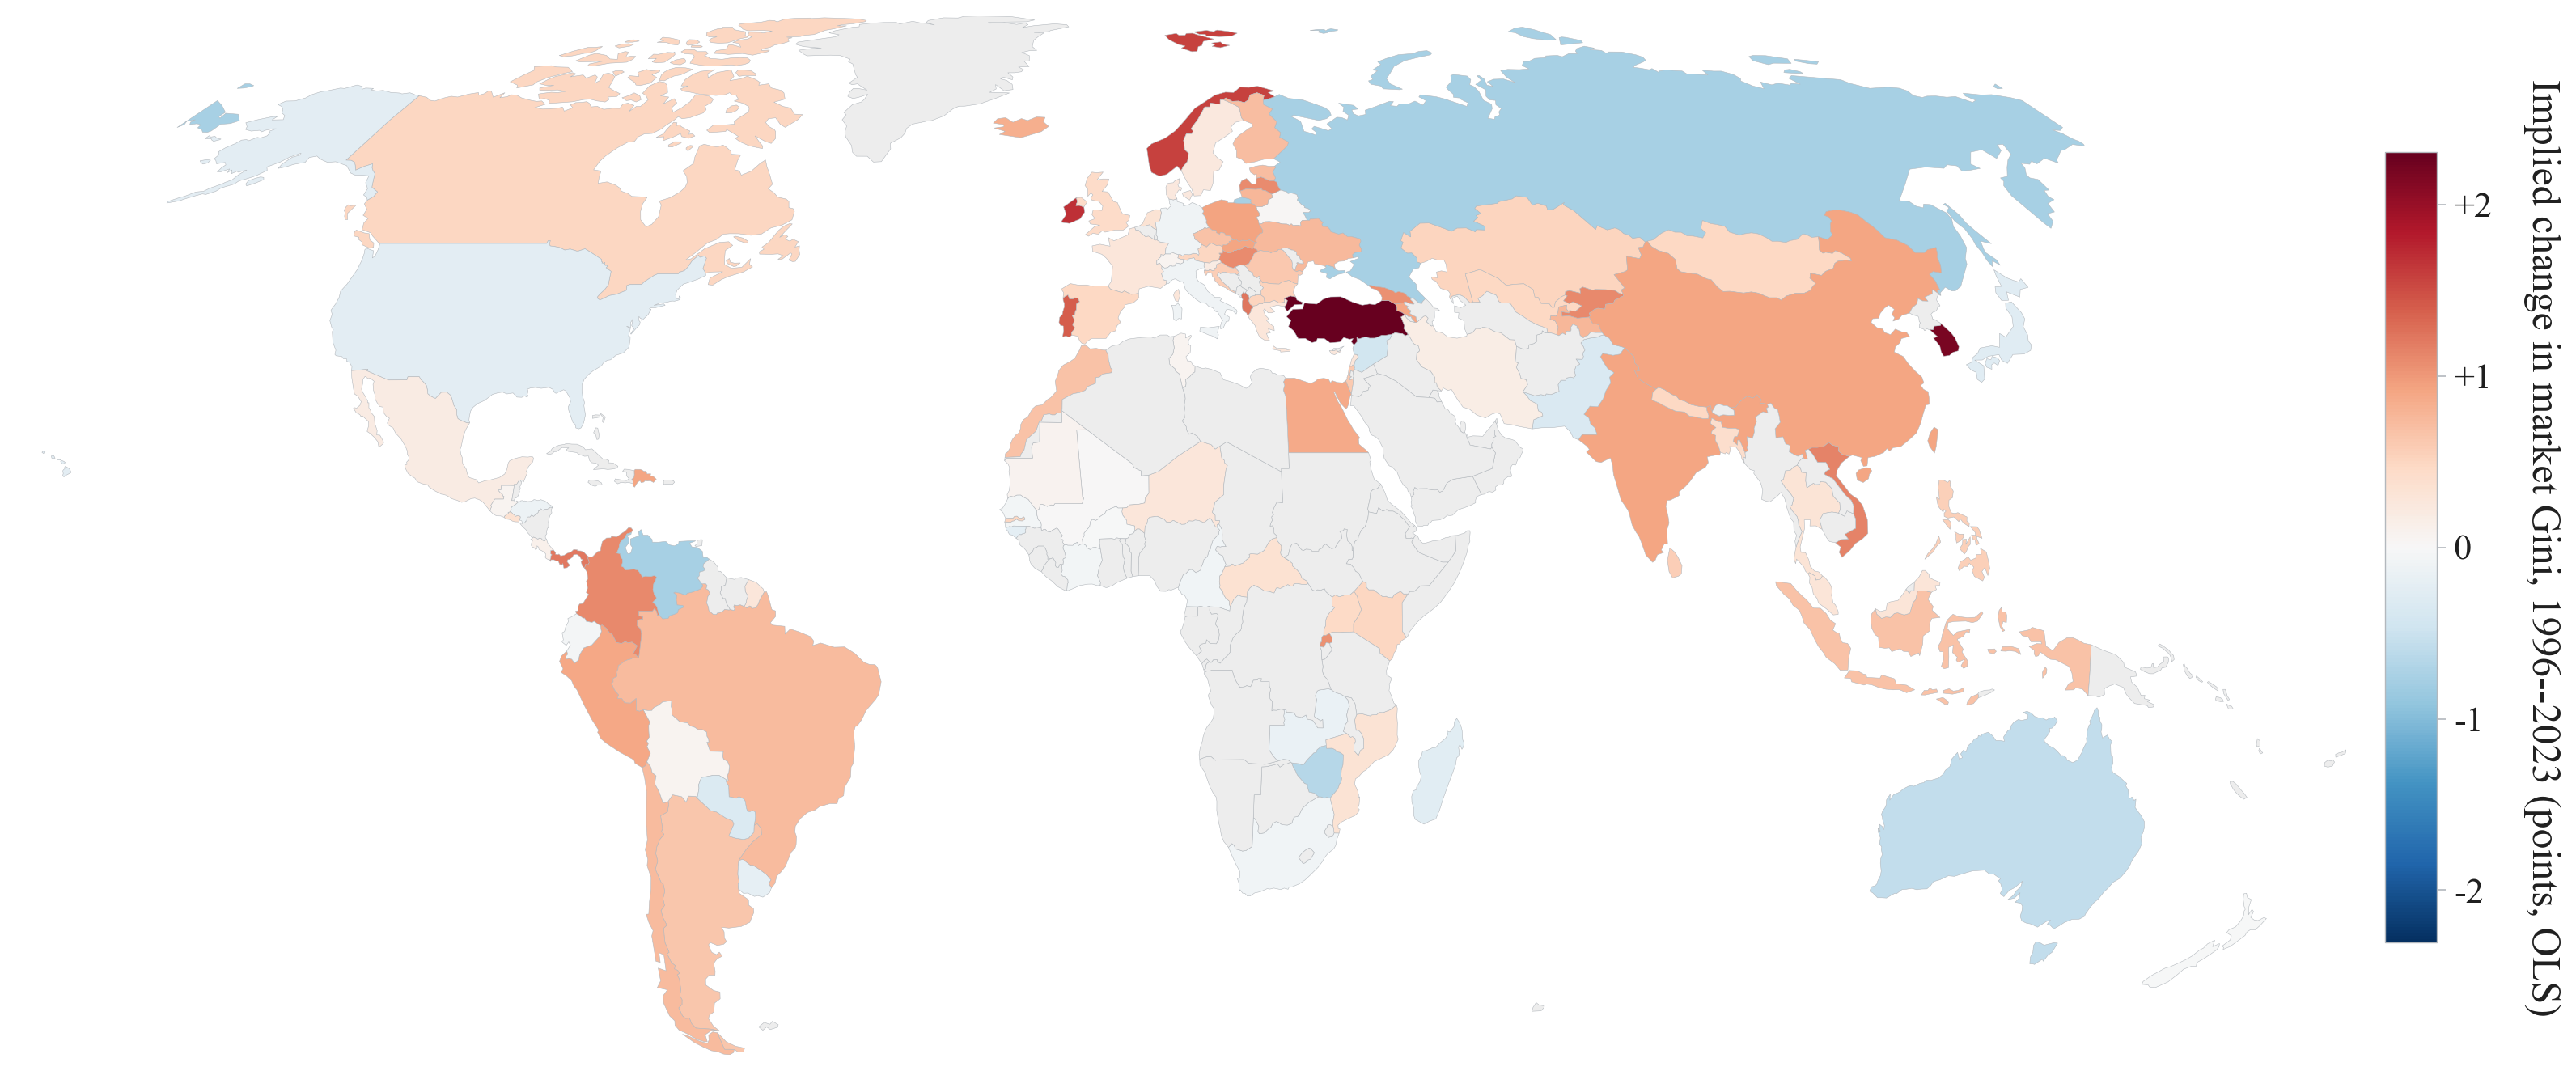
\includegraphics[width=\linewidth]{fig_map_implied_gini.png}
\caption{Implied change in the market Gini from hub-connectivity growth, 1996--2023, in points. The OLS coefficient ($0.061$) is applied to each country's change in $\ln\mathrm{GACI}_{max}$ between its first and last observation. Grey denotes economies not observed in both 1996--1998 and 2019--2023.}\label{fig:map_implied}\end{figure}

\section{Identification diagnostics and robustness}
\label{sec:diag}
Because both instruments are shift-share interactions with a single global shifter, the credibility of the 2SLS estimates depends on baseline exposure being unrelated to differential inequality trends. We conduct three sets of checks to address the concerns that (i) the exposure variable proxies for continent-level or income-group-level inequality trends, (ii) the instruments identify the level of connectivity but not its change, and (iii) the estimate is sensitive to specification and sample.

\subsection{Exposure-trend diagnostics}
Table~\ref{tab:diag} tightens the fixed-effects structure in steps. First, because a continent-level inequality trend correlated with baseline air market access would violate the exclusion restriction, we add continent by year fixed effects; the market-Gini estimate is $0.48$ with either instrument. Second, because other baseline characteristics may carry their own trends, we add baseline income, inequality, land area, latitude and sea market access, each interacted with the aviation index; the estimate falls to $0.38$ (Feyrer) and $0.44$ (tourism) with year fixed effects and to $0.28$ and $0.23$ with continent by year fixed effects. Third, income tercile and inequality tercile by year fixed effects give $0.34$ and $0.40$. With all of these together the Feyrer estimate is $0.33$ ($p<0.01$) and the tourism estimate $0.21$ ($p=0.13$); both instruments jointly, with continent by year fixed effects and exposure controls, give $0.31$ ($p<0.01$) with a Hansen $J$ $p$-value of $0.95$. The OLS estimate with the full interacted fixed-effects structure is $0.025$ ($p<0.01$). The market-Gini result is therefore not an artefact of continent-level or income-group-level inequality trends, although its magnitude falls by about a third once other exposures are allowed their own trends.

The disposable-Gini result is less robust. It is $0.13$ and not significant with continent by year fixed effects under the Feyrer instrument, $0.05$ with exposure controls and continent by year effects, and $0.08$ in the full specification; the tourism instrument gives $0.34$ ($p=0.03$) in the full specification, and the two instruments are rejected jointly ($J$ $p=0.04$). We therefore treat the market-income result as the finding and the disposable-income result as suggestive.

The first stage differs in sign across continents. Baseline air market access predicts faster hub-connectivity growth in Africa (first-stage coefficient $0.37$) and slower growth in Asia, Europe and Latin America ($-0.23$, $-0.33$ and $-0.21$), a pattern consistent with convergence within the already-connected continents and catch-up in Africa. The pooled first stage is positive because it combines within-continent and between-continent variation, and the reduced form inherits the same sign pattern (Table~\ref{tab:a_rfcont}). Sign heterogeneity in the first stage implies that the pooled 2SLS estimate is not a convex average of continent-specific effects, which is a further reason to prefer the continent by year specification and to report the continent-specific estimates in Table~\ref{tab:hetero}.

Dropping one continent at a time under continent by year fixed effects leaves the market estimate between $0.27$ and $0.58$ and significant, except when Asia is dropped and the first stage becomes weak. Under year fixed effects only, dropping Latin America reverses the sign, because Latin America combines low baseline air market access with the largest inequality decline in the sample; the reversal disappears once continent by year effects are included ($0.58$, $p<0.01$).

\begin{table}[H]\centering\caption{Identification diagnostics for the shift-share instruments.}\label{tab:diag}
\begin{threeparttable}\small\begin{tabular}{lcccc}
\toprule
Specification & Instrument & $\ln G^{mkt}$ & $\ln G^{disp}$ & KP $F$ \\
\midrule
Continent $\times$ year FE & Feyrer & 0.483\sym{***} (0.142) & 0.126 (0.109) & 16.7 \\
 & Tourism & 0.476\sym{**} (0.206) & 0.337\sym{*} (0.177) & 8.6 \\
Continent $\times$ year FE, drop Latin America & Feyrer & 0.579\sym{***} (0.181) & 0.238\sym{*} (0.135) & 12.3 \\
 & Tourism & 0.787\sym{*} (0.467) & 0.636 (0.404) & 3.1 \\
+ baseline exposures $\times$ aviation index & Feyrer & 0.377\sym{***} (0.063) & 0.506\sym{***} (0.077) & 79.4 \\
 & Tourism & 0.443\sym{***} (0.132) & 0.580\sym{***} (0.153) & 19.7 \\
+ exposures $\times$ index, continent $\times$ year FE & Feyrer & 0.275\sym{***} (0.103) & 0.048 (0.102) & 22.5 \\
 & Tourism & 0.232 (0.171) & 0.424\sym{*} (0.224) & 6.8 \\
Income tercile and Gini tercile $\times$ year FE & Feyrer & 0.342\sym{***} (0.056) & 0.484\sym{***} (0.071) & 86.0 \\
 & Tourism & 0.403\sym{***} (0.150) & 0.327\sym{**} (0.141) & 12.5 \\
All of the above & Feyrer & 0.334\sym{***} (0.117) & 0.083 (0.111) & 17.5 \\
 & Tourism & 0.205 (0.135) & 0.344\sym{**} (0.162) & 10.7 \\
Exposures $\times$ index, continent $\times$ year FE & Both & 0.306\sym{***} (0.103) & 0.214\sym{**} (0.101) & 12.8 \\
\quad Hansen $J$ $p$-value & & 0.95 & 0.04 & \\
OLS with all interacted FE & -- & 0.025\sym{***} (0.008) & 0.010 (0.009) & \\
\addlinespace\multicolumn{5}{l}{\emph{First stage by continent (coefficient on instrument, KP $F$)}}\\
Africa & Feyrer / Tourism & 0.365\sym{***} [40.6] & -0.018 [1.0] & \\
Asia & Feyrer / Tourism & -0.234\sym{***} [27.2] & 0.069\sym{**} [4.3] & \\
Europe & Feyrer / Tourism & -0.332\sym{***} [43.5] & -0.024 [1.7] & \\
Latin America & Feyrer / Tourism & -0.208\sym{**} [5.5] & 0.067\sym{***} [20.1] & \\
Middle East & Feyrer / Tourism & -0.451 [1.1] & 0.033 [0.3] & \\
North America & Feyrer / Tourism & 0.165 [1.1] & 0.072\sym{***} [11.3] & \\
Oceania & Feyrer / Tourism & -0.006 [0.0] & 0.123\sym{***} [51.7] & \\
\bottomrule
\end{tabular}
\begin{tablenotes}\footnotesize\item Robust SE in parentheses. Exposures interacted with the aviation index $a_t$: baseline ln GDP per capita, baseline market Gini, ln land area, absolute latitude and ln sea market access. \sym{*}~$p<0.10$, \sym{**}~$p<0.05$, \sym{***}~$p<0.01$.\end{tablenotes}\end{threeparttable}\end{table}

\subsection{Horizon, long differences and liberalisation episodes}
\label{sec:horizon}
The panel estimates are contemporaneous, so we next ask whether they reflect the timing of a response or the persistence of the series. Table~\ref{tab:horizon} and Figure~\ref{fig:horizon} examine the horizon. The 2SLS coefficient on connectivity lagged one to ten years is stable between $0.40$ and $0.52$, and the coefficient on connectivity led one to five years is as large or larger. A joint specification with current and three-year-ahead connectivity is uninformative because the two instruments are nearly collinear; Table~\ref{tab:a_leads} reports the lead coefficients. The lead pattern is what a persistent regressor and a trending instrument produce, and it does not distinguish anticipation from persistence.

Long differences are the natural design for a slow-moving outcome, and they are where the instruments lose power. In cross-sections of changes over 1996--2019, 2000--2019, 2005--2019 and 2010--2019 with continent fixed effects, the OLS coefficient is positive and imprecise ($0.03$ to $0.07$ for the market Gini). The first stage of the differenced Feyrer instrument is weak in every window, as is that of the differenced tourism instrument; stacked five-year differences give an estimate of $0.06$ ($p=0.46$) with the tourism instrument. The instruments therefore predict the level of connectivity within countries, through the interaction of a trending shifter with fixed exposure, but not its medium-run change. The 2SLS evidence is evidence on within-country co-movement, not on the response to discrete connectivity shocks.

Bilateral liberalisation is the third design. We collected the year in which each of 139 Open Skies agreements with the United States was first applied and estimate staggered difference-in-differences and event-study specifications, excluding the thirteen economies treated before 1997 (Table~\ref{tab:openskies}). Open Skies application does not move the connectivity measures: the post-treatment coefficient on ln hub connectivity is $0.02$ ($p=0.15$) and the event-study coefficients rise slowly to $0.05$ ten years after application without becoming significant. The market Gini rises by $0.024$ log points after application, but the event study shows a monotone pre-trend from $-0.018$ six years before to $-0.008$ one year before, so the post-treatment coefficients continue a trend rather than break one. The Callaway--Sant'Anna estimator with not-yet-treated controls gives the same result: an average treatment effect of $0.025$ ($p=0.22$) on ln hub connectivity and $0.017$ ($p=0.07$) on the market Gini. The event-study coefficients are reported in Tables~\ref{tab:a_es_conn} and \ref{tab:a_es_ineq}. As an instrument, Open Skies is weak; used together with the Feyrer instrument in an over-identified specification it gives a market-Gini coefficient of $0.427$ (Table~\ref{tab:a_osfeyrer}). The liberalisation design therefore neither confirms nor overturns the panel result.

\begin{figure}[H]\centering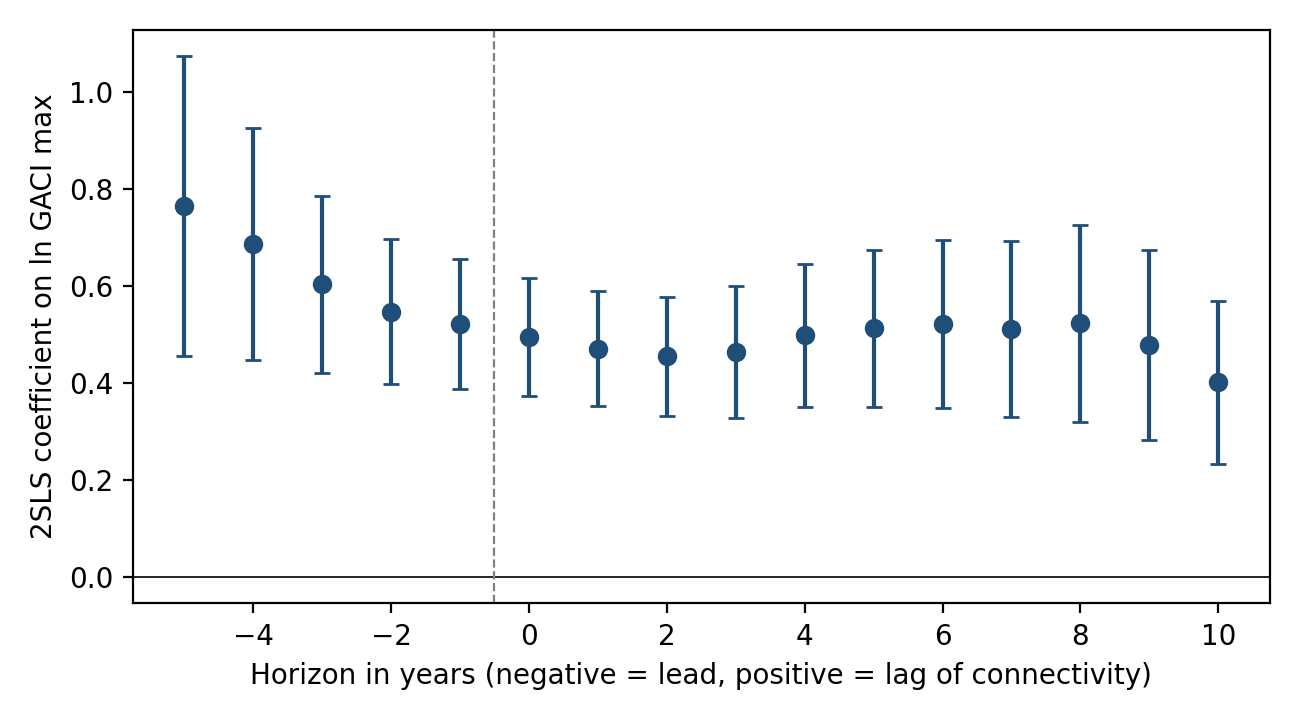
\includegraphics[width=0.75\textwidth]{fig_horizon.png}
\caption{2SLS coefficient on hub connectivity by horizon, market Gini, Feyrer instrument. Negative horizons are leads of connectivity; positive horizons are lags. Bars are 95 percent robust confidence intervals.}\label{fig:horizon}\end{figure}

\begin{table}[H]\centering\caption{Timing: lagged connectivity, long differences and stacked differences.}\label{tab:horizon}
\begin{threeparttable}\small\begin{tabular}{lcccc}
\toprule
Specification & $\ln G^{mkt}$ & $\ln G^{disp}$ & KP $F$ & N \\
\midrule
\multicolumn{5}{l}{\emph{Panel A. Lagged connectivity, 2SLS (instrument lagged equally)}}\\
Lag 0 & 0.495\sym{***} (0.062) & 0.651\sym{***} (0.077) & 98.5 & 3,735 \\
Lag 1 & 0.471\sym{***} (0.061) & 0.623\sym{***} (0.075) & 94.0 & 3,568 \\
Lag 2 & 0.455\sym{***} (0.063) & 0.617\sym{***} (0.078) & 86.0 & 3,401 \\
Lag 3 & 0.464\sym{***} (0.070) & 0.645\sym{***} (0.088) & 76.4 & 3,236 \\
Lag 5 & 0.513\sym{***} (0.082) & 0.712\sym{***} (0.105) & 63.6 & 2,912 \\
Lag 7 & 0.511\sym{***} (0.092) & 0.721\sym{***} (0.122) & 47.2 & 2,604 \\
Lag 10 & 0.402\sym{***} (0.086) & 0.588\sym{***} (0.112) & 38.3 & 2,144 \\
\addlinespace\multicolumn{5}{l}{\emph{Panel B. Long differences, cross-section with continent FE}}\\
1996--2019, OLS & 0.066 (0.045) & 0.026 (0.040) &  & 102 \\
1996--2019, 2SLS Feyrer & 1.749 (3.929) & 0.984 (2.329) & 0.16 & 102 \\
1996--2019, 2SLS tourism & 39.210 (1566.961) & 21.475 (857.209) & 0.00 & 102 \\
2000--2019, OLS & 0.056 (0.043) & 0.018 (0.036) &  & 106 \\
2000--2019, 2SLS Feyrer & 0.836 (0.986) & 0.358 (0.653) & 0.63 & 106 \\
2000--2019, 2SLS tourism & 2.201 (4.801) & 1.278 (2.964) & 0.18 & 106 \\
2005--2019, OLS & 0.055 (0.039) & 0.003 (0.039) &  & 114 \\
2005--2019, 2SLS Feyrer & 0.421 (0.370) & 0.074 (0.329) & 2.05 & 114 \\
2005--2019, 2SLS tourism & 0.647 (0.436) & 0.346 (0.337) & 2.91 & 114 \\
2010--2019, OLS & -0.043 (0.041) & -0.084\sym{*} (0.047) &  & 120 \\
2010--2019, 2SLS Feyrer & 1.921 (11.829) & 2.525 (15.596) & 0.03 & 120 \\
2010--2019, 2SLS tourism & 1.898 (3.340) & 0.643 (1.480) & 0.35 & 120 \\
Stacked 5-year differences, OLS & -0.007 (0.011) & -0.020 (0.014) &  & 2,914 \\
Stacked 5-year differences, 2SLS tourism & 0.063 (0.086) & 0.066 (0.089) & 12.79 & 2,914 \\
\bottomrule
\end{tabular}
\begin{tablenotes}\footnotesize\item Panel A: country and year fixed effects, robust SE. Panel B: cross-sections of changes with continent fixed effects, robust SE; stacked five-year differences with year and continent effects and country-clustered SE. \sym{*}~$p<0.10$, \sym{**}~$p<0.05$, \sym{***}~$p<0.01$.\end{tablenotes}\end{threeparttable}\end{table}

\begin{table}[H]\centering\caption{Open Skies agreements: staggered difference-in-differences and instrument.}\label{tab:openskies}
\begin{threeparttable}\small\begin{tabular}{lcccc}
\toprule
Outcome & DiD, country and year FE & DiD, continent $\times$ year FE & Pre-trend joint $F$ ($p$) & N \\
\midrule
ln GACI max & 0.020 (0.014) & 0.008 (0.012) & 1.56 (0.17) & 3,389 \\
ln GACI cwm & 0.017 (0.012) & 0.005 (0.010) & 1.69 (0.14) & 3,389 \\
ln GACI sum & 0.039 (0.042) & 0.016 (0.041) & 1.05 (0.39) & 3,389 \\
ln Gini, market & 0.024\sym{***} (0.007) & 0.014\sym{**} (0.006) & 2.90 (0.02) & 3,389 \\
ln Gini, disposable & 0.024\sym{***} (0.008) & 0.016\sym{**} (0.007) & 3.04 (0.01) & 3,389 \\
ln bottom 50\% share & -0.007 (0.018) & -0.005 (0.018) & 0.93 (0.46) & 3,368 \\
ln top 10\% share & 0.003 (0.010) & 0.005 (0.010) & 3.07 (0.01) & 3,368 \\
\addlinespace\multicolumn{5}{l}{\emph{Open Skies as instrument for ln GACI max (2SLS, clustered SE)}}\\
ln Gini, market & 1.195 (0.805) [KP $F$ 2.1] & 1.773 (2.739) & & 3,389 \\
ln Gini, disposable & 1.176 (0.796) [KP $F$ 2.1] & 2.066 (3.157) & & 3,389 \\
ln bottom 50\% share & -0.315 (0.859) [KP $F$ 2.2] & -0.682 (2.438) & & 3,368 \\
ln top 10\% share & 0.159 (0.484) [KP $F$ 2.2] & 0.635 (1.581) & & 3,368 \\
\bottomrule
\end{tabular}
\begin{tablenotes}\footnotesize\item Treatment is the year an Open Skies agreement with the United States was first applied; economies treated before 1997 are excluded. Country-clustered SE. Pre-trend $F$ tests the joint significance of event-time coefficients $-6$ to $-2$. \sym{*}~$p<0.10$, \sym{**}~$p<0.05$, \sym{***}~$p<0.01$.\end{tablenotes}\end{threeparttable}\end{table}

\subsection{Robustness}
Table~\ref{tab:robust} reports the remaining checks. First, because the baseline controls only for population, we add GDP per capita, urbanisation, tertiary enrolment, trade, tax revenue or sea market access; the market estimate remains between $0.49$ and $0.81$, and the increase with GDP per capita is the suppression documented in Table~\ref{tab:mech}. Second, because inference with seven continent clusters is imprecise, we compare clustering schemes; two-way clustering by continent and year widens the confidence interval to include zero, whereas Driscoll--Kraay errors give $p<0.01$. Third, because the leading hubs and the crisis years may drive the estimate, we drop the ten leading hub economies ($0.57$), restrict the sample to 1996--2019 ($0.44$) and drop 2008--09 and 2020--21 ($0.48$); the estimate is robust. Fourth, country-specific linear trends remove the identifying variation of an instrument that is nearly linear in time and give an uninformative estimate. Fifth, the survey-based World Bank Gini and decile shares, available for 1,877 country-years, give the same signs in both OLS and 2SLS: the Gini and the top-decile share rise and the bottom-quintile share falls.

Figure~\ref{fig:rfq} shows the reduced form by quintile of baseline inequality and baseline income. The reduced-form coefficient of the Feyrer instrument on the market Gini is positive in every income quintile except the richest, where it is zero, and positive in the second, fourth and fifth baseline-inequality quintiles. The association is therefore not driven by the richest or by the most unequal economies.

\begin{table}[H]\centering\caption{Robustness of the hub-connectivity estimate (2SLS, Feyrer instrument).}\label{tab:robust}
\begin{threeparttable}\small\begin{tabular}{lcccc}
\toprule
Specification & $\ln G^{mkt}$ & $\ln G^{disp}$ & KP $F$ / Hansen $p$ & N \\
\midrule
Baseline (ln population) & 0.495\sym{***} (0.062) & 0.651\sym{***} (0.077) & 98.5 & 3,735 \\
+ ln GDP per capita & 0.753\sym{***} (0.109) & 0.968\sym{***} (0.140) & 55.9 & 3,735 \\
+ urban share & 0.504\sym{***} (0.063) & 0.663\sym{***} (0.078) & 98.1 & 3,735 \\
+ tertiary enrolment & 0.546\sym{***} (0.137) & 0.757\sym{***} (0.169) & 26.0 & 2,508 \\
+ trade/GDP & 0.486\sym{***} (0.062) & 0.651\sym{***} (0.078) & 92.5 & 3,725 \\
+ tax/GDP & 0.667\sym{***} (0.160) & 0.899\sym{***} (0.196) & 28.5 & 2,595 \\
+ ln sea market access & 0.535\sym{***} (0.071) & 0.718\sym{***} (0.089) & 88.6 & 3,735 \\
+ GDP pc, urban, tertiary, trade & 0.814\sym{***} (0.263) & 1.118\sym{***} (0.337) & 12.4 & 2,500 \\
Both instruments (Hansen $J$ $p$ in col. 4) & 0.490\sym{***} (0.055) & 0.606\sym{***} (0.064) & 67.5 / 0.88 & 3,735 \\
Tourism instrument only & 0.468\sym{***} (0.165) & 0.391\sym{***} (0.151) & 13.6 & 3,735 \\
SE clustered by country & 0.495\sym{**} (0.194) & 0.651\sym{***} (0.241) & 10.6 & 3,735 \\
SE two-way clustered continent, year & 0.495 (0.424) & 0.651 (0.471) & 15.6 & 3,735 \\
Driscoll--Kraay SE (3 lags) & 0.495\sym{***} (0.069) & 0.651\sym{***} (0.096) & 20.2 & 3,735 \\
Drop ten leading hub economies & 0.565\sym{***} (0.066) & 0.709\sym{***} (0.082) & 94.0 & 3,472 \\
1996--2019 only & 0.439\sym{***} (0.052) & 0.574\sym{***} (0.064) & 118.6 & 3,344 \\
Drop 2008--09 and 2020--21 & 0.480\sym{***} (0.056) & 0.635\sym{***} (0.071) & 114.9 & 3,204 \\
Continent $\times$ year FE & 0.483\sym{***} (0.142) & 0.126 (0.109) & 16.7 & 3,734 \\
Country-specific linear trends & -0.740 (0.652) & -0.808 (0.740) & 1.3 & 3,735 \\
\addlinespace\multicolumn{5}{l}{\emph{Leave-one-continent-out (country and year FE)}}\\
Drop Africa & 0.683\sym{***} (0.094) & 0.885\sym{***} (0.120) & 63.9 & 2,790 \\
Drop Asia & 0.712\sym{***} (0.092) & 0.824\sym{***} (0.107) & 76.2 & 3,110 \\
Drop Europe & 0.313\sym{***} (0.057) & 0.504\sym{***} (0.078) & 56.6 & 2,604 \\
Drop Latin America & -0.080\sym{**} (0.041) & 0.010 (0.037) & 78.6 & 3,179 \\
Drop Middle East & 0.603\sym{***} (0.080) & 0.787\sym{***} (0.101) & 80.5 & 3,498 \\
Drop North America & 0.568\sym{***} (0.069) & 0.733\sym{***} (0.087) & 88.0 & 3,658 \\
Drop Oceania & 0.576\sym{***} (0.076) & 0.774\sym{***} (0.097) & 80.2 & 3,571 \\
\bottomrule
\end{tabular}
\begin{tablenotes}\footnotesize\item Robust SE in parentheses unless the row states otherwise. \sym{*}~$p<0.10$, \sym{**}~$p<0.05$, \sym{***}~$p<0.01$.\end{tablenotes}\end{threeparttable}\end{table}

\begin{figure}[H]\centering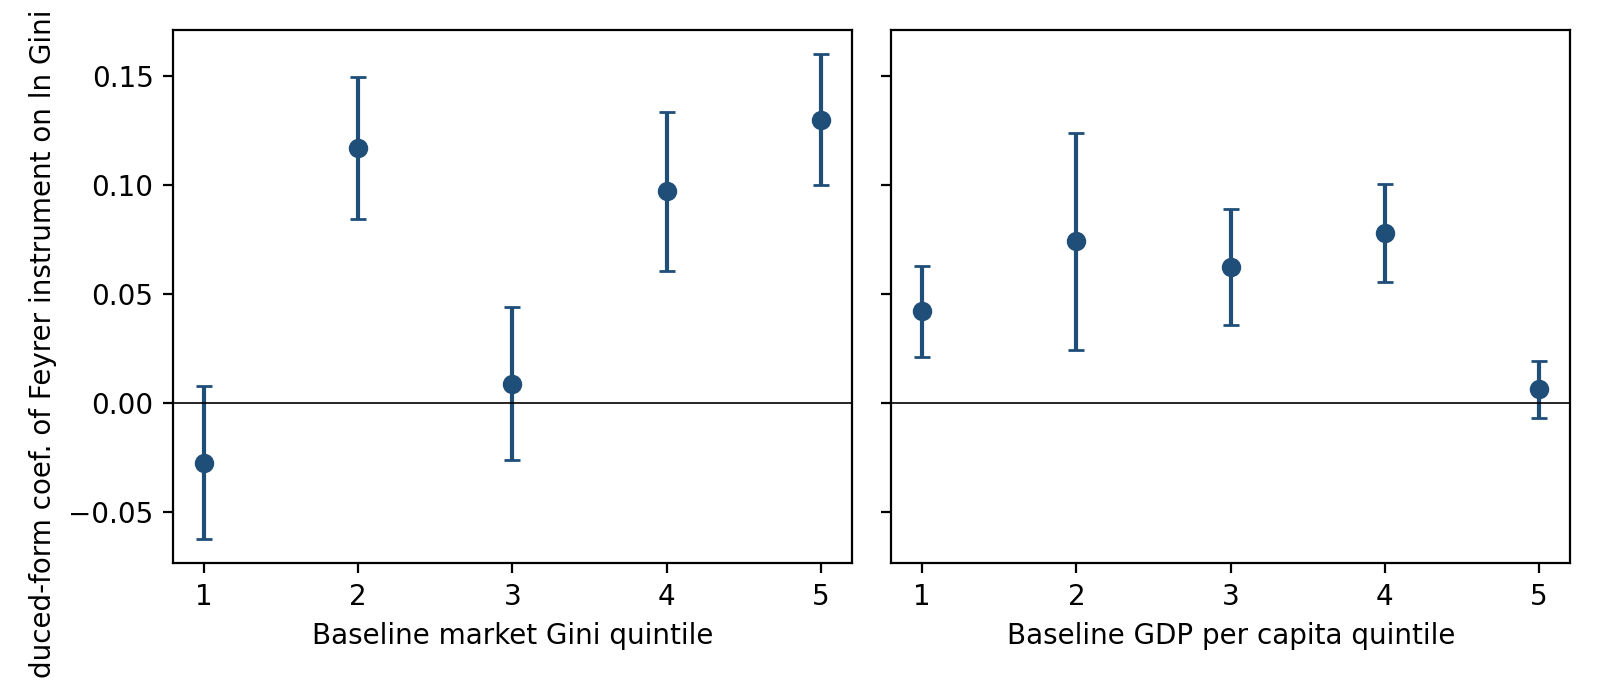
\includegraphics[width=0.85\textwidth]{fig_rf_quintile.png}
\caption{Reduced-form coefficient of the Feyrer instrument on the market Gini by quintile of baseline inequality (left) and baseline income (right). Country and year fixed effects; 95 percent robust confidence intervals.}\label{fig:rfq}\end{figure}

\section{Synthesis: the hypotheses revisited}
\label{sec:synthesis}
First, Hypothesis~1 is supported for market inequality and not for attenuation by redistribution. Within countries, rising hub connectivity accompanies a rising market Gini in OLS, in 2SLS with two different instruments, and under continent by year and income-group by year fixed effects. The disposable Gini rises by at least as much, and the redistribution wedge narrows.

Second, Hypothesis~2 is supported at the bottom half and the top decile and rejected at the top percentile. The pretax income share of the bottom half falls, the top decile share rises by less, and the top percentile share does not move. The distributional response to connectivity is a widening between the upper-middle of the distribution and the bottom half rather than an increase at the very top. Measured in levels, the same result is an average income gain of which the bottom half retains about one third, and the ratio of top-decile to bottom-half average income is the one growth quantity that survives the continent by year and over-identification checks.

Third, Hypothesis~3 is supported. At a given total connectivity, a network concentrated in one gateway is associated with higher inequality and dispersion across airports with lower inequality, and the marginal gateway gain is associated with the largest increase in inequality where the network was previously distributed.

Fourth, Hypothesis~4 is supported. Connectivity raises income, industrial employment and urbanisation, each of which is associated with lower inequality, so the residual association is larger than the total; unemployment is the only channel that operates in the same direction.

Two qualifications bound these conclusions. First, the 2SLS magnitudes are too large to be structural elasticities, as the aggregate contribution exercise shows, and the relevant order of magnitude is the OLS one: about half a Gini point for the average country's connectivity growth since 1996. Second, neither long differences nor liberalisation episodes move connectivity with sufficient precision, so the evidence is on co-movement within countries rather than on the response to identified shocks.

\section{Conclusion}
\label{sec:conclusion}
Gateway connectivity is associated with growth, and this paper asks who receives it. Using a global panel of 166 economies over 1996--2023, we find that within-country increases in the connectivity of the primary hub accompany increases in market-income inequality, located in a falling income share of the bottom half and a rising share of the top decile, with no response at the top percentile. The association is present under continent by year and income-group by year fixed effects, is larger in Asia and after 2010, is reversed in Africa, and is larger in networks where connectivity is concentrated in a single gateway at a given total. It is not a by-product of growth: the income, industrial employment and urbanisation that connectivity induces are associated with lower inequality, and the residual association is larger than the total.

The policy reading follows the companion paper's distinction between hub concentration and distributed access. If the objective is the aggregate, the gateway is where the return to connectivity is largest; if the objective includes the distribution, the same connectivity spread across secondary airports is associated with a smaller increase in inequality. The evidence is on co-movement rather than on shock responses, and the next step is subnational: airport-level connectivity matched to local income and night-light data would identify whether the gateway region's gain is offset elsewhere in the country, which is the mechanism that this paper's national estimates imply but cannot observe.

\appendix
%=======================================================================
\section{Additional estimates}
\label{app:additional}
%=======================================================================
The tables in the body report the log specification for hub connectivity. This appendix reports the remaining estimates produced by the same estimation scripts: the Gini in points, absolute redistribution, the distributional shares for the other two connectivity measures, the income-tercile splits, the continent-specific estimates for both measures, and the survey-based outcomes.

Table~\ref{tab:a_levels} repeats Table~\ref{tab:main} with the Gini in points rather than in logs. A one-log-point increase in hub connectivity is associated with 2.5 Gini points in OLS and 24.1 points in 2SLS with the Feyrer instrument. The 2SLS magnitude in points is the quantity compared with observed changes in Section~\ref{sec:contrib}, where it is found to exceed any change observed in the sample.

\begin{table}[H]\centering\caption{Main results with the Gini measured in points.}\label{tab:a_levels}
\begin{threeparttable}\small\begin{tabular}{lcc}
\toprule
 & Market Gini & Disposable Gini \\
 & (points) & (points) \\
\midrule
\multicolumn{3}{l}{\emph{Panel A. Hub connectivity, $\ln\mathrm{GACI}_{max}$}}\\
OLS & 2.463\sym{***} (0.339) & 2.460\sym{***} (0.343) \\
2SLS, Feyrer IV & 24.076\sym{***} (2.971) & 30.086\sym{***} (3.487) \\
 & [9.351]\sym{**} & [10.979]\sym{***} \\
2SLS, tourism IV & 20.298\sym{***} (7.414) & 14.540\sym{**} (5.811) \\
 & [11.958]\sym{*} & [11.457] \\
\addlinespace
\multicolumn{3}{l}{\emph{Panel B. Hub quality, $\ln\mathrm{GACI}_{cwm}$}}\\
OLS & 3.186\sym{***} (0.381) & 2.860\sym{***} (0.379) \\
2SLS, Feyrer IV & 28.951\sym{***} (3.677) & 36.177\sym{***} (4.358) \\
 & [11.655]\sym{**} & [13.757]\sym{***} \\
2SLS, tourism IV & 31.506\sym{**} (13.937) & 22.567\sym{**} (10.756) \\
 & [24.498] & [20.879] \\
\addlinespace
\multicolumn{3}{l}{\emph{Panel C. Total connectivity, $\ln\mathrm{GACI}_{sum}$}}\\
OLS & 0.351\sym{***} (0.106) & 0.527\sym{***} (0.124) \\
2SLS, Feyrer IV & 9.670\sym{***} (1.215) & 12.084\sym{***} (1.369) \\
 & [3.601]\sym{***} & [3.985]\sym{***} \\
2SLS, tourism IV & 11.273\sym{**} (4.419) & 8.075\sym{**} (3.492) \\
 & [8.591] & [7.238] \\
\midrule
Country, Year FE & Yes & Yes \\
Observations & 3,735 & 3,735 \\
\bottomrule
\end{tabular}
\begin{tablenotes}\footnotesize\item Robust SE in parentheses; country-clustered SE in brackets with the corresponding significance level. Country and year fixed effects and log population throughout. First stages are those of Table~\ref{tab:main}. \sym{*}~$p<0.10$, \sym{**}~$p<0.05$, \sym{***}~$p<0.01$.\end{tablenotes}\end{threeparttable}\end{table}

Table~\ref{tab:a_absred} reports absolute redistribution, the difference between the market and disposable Gini in points, as an outcome. The OLS coefficients are not distinguishable from zero. The 2SLS coefficients with the Feyrer instrument are negative and significant under robust errors for all three connectivity measures, and none is significant under country-clustered errors. The tourism instrument is uninformative for this outcome, with a first-stage $F$ of $0.02$ for hub quality. The sample is 1,898 country-years, about half the estimation sample, because the wedge requires both series to be observed.

\begin{table}[H]\centering\caption{Absolute redistribution (market minus disposable Gini, points) as an outcome.}\label{tab:a_absred}
\begin{threeparttable}\small\begin{tabular}{lccc}
\toprule
Connectivity measure & OLS & 2SLS, Feyrer IV & 2SLS, tourism IV \\
\midrule
Hub connectivity, $\ln\mathrm{GACI}_{max}$ & -0.119 (0.319) & -5.639\sym{***} (1.643) & 20.150 (25.481) \\
 & & [5.191] & [41.665] \\
Hub quality, $\ln\mathrm{GACI}_{cwm}$ & 0.122 (0.369) & -6.745\sym{***} (1.936) & 164.648 (1240.821) \\
 & & [6.071] & [2162.857] \\
Total connectivity, $\ln\mathrm{GACI}_{sum}$ & -0.053 (0.102) & -3.194\sym{***} (0.950) & 4.710 (3.771) \\
 & & [2.918] & [7.789] \\
\midrule
Observations & 1,898 & 1,898 & 1,898 \\
\bottomrule
\end{tabular}
\begin{tablenotes}\footnotesize\item Robust SE in parentheses; country-clustered SE in brackets. OLS does not depend on the instrument and is reported once. \sym{*}~$p<0.10$, \sym{**}~$p<0.05$, \sym{***}~$p<0.01$.\end{tablenotes}\end{threeparttable}\end{table}

Table~\ref{tab:a_tails_other} reports the distributional shares of Table~\ref{tab:tails} for hub quality and total connectivity. The signs match the hub-connectivity results: the bottom-half share falls, the top-decile share rises and the top-percentile share does not respond.

\begin{table}[H]\centering\caption{Distributional location for hub quality and total connectivity (Feyrer instrument).}\label{tab:a_tails_other}
\begin{threeparttable}\small\begin{tabular}{lccc}
\toprule
Outcome & OLS & 2SLS (robust SE) & 2SLS (clustered SE) \\
\midrule
\multicolumn{4}{l}{\emph{Panel A. Hub quality, $\ln\mathrm{GACI}_{cwm}$}}\\
Top 10\% share (pretax) & 0.065\sym{***} (0.016) & 0.269\sym{***} (0.076) & 0.269 (0.228) \\
Top 1\% share (pretax) & 0.201\sym{***} (0.036) & 0.080 (0.158) & 0.080 (0.458) \\
Bottom 50\% share (pretax) & -0.052\sym{**} (0.023) & -0.929\sym{***} (0.165) & -0.929\sym{*} (0.508) \\
ln(top 10\% / bottom 50\%) & 0.118\sym{***} (0.037) & 1.197\sym{***} (0.231) & 1.197\sym{*} (0.709) \\
Gini, pretax (WID) & 0.046\sym{***} (0.013) & 0.261\sym{***} (0.063) & 0.261 (0.192) \\
Gini, post-tax (WID) & 0.063\sym{***} (0.015) & 0.461\sym{***} (0.084) & 0.461\sym{*} (0.251) \\
Top 10\% share (post-tax) & 0.075\sym{***} (0.016) & 0.484\sym{***} (0.094) & 0.484\sym{*} (0.272) \\
Bottom 50\% share (post-tax) & -0.103\sym{***} (0.020) & -1.308\sym{***} (0.184) & -1.308\sym{**} (0.570) \\
Top 10\% share, levels & 0.026\sym{***} (0.006) & 0.118\sym{***} (0.035) & 0.118 (0.105) \\
Top 1\% share, levels & 0.027\sym{***} (0.005) & -0.014 (0.029) & -0.014 (0.085) \\
Bottom 50\% share, levels & -0.010\sym{***} (0.004) & -0.098\sym{***} (0.020) & -0.098 (0.061) \\
KP $F$ (2SLS) & & 82.7 & \\
\addlinespace
\multicolumn{4}{l}{\emph{Panel B. Total connectivity, $\ln\mathrm{GACI}_{sum}$}}\\
Top 10\% share (pretax) & 0.006 (0.004) & 0.091\sym{***} (0.026) & 0.091 (0.080) \\
Top 1\% share (pretax) & 0.018\sym{**} (0.008) & 0.027 (0.054) & 0.027 (0.158) \\
Bottom 50\% share (pretax) & -0.006 (0.006) & -0.316\sym{***} (0.053) & -0.316\sym{**} (0.160) \\
ln(top 10\% / bottom 50\%) & 0.013 (0.010) & 0.407\sym{***} (0.075) & 0.407\sym{*} (0.233) \\
Gini, pretax (WID) & 0.005 (0.003) & 0.089\sym{***} (0.021) & 0.089 (0.065) \\
Gini, post-tax (WID) & 0.009\sym{**} (0.004) & 0.157\sym{***} (0.027) & 0.157\sym{*} (0.083) \\
Top 10\% share (post-tax) & 0.011\sym{***} (0.004) & 0.165\sym{***} (0.031) & 0.165\sym{*} (0.093) \\
Bottom 50\% share (post-tax) & -0.011\sym{*} (0.006) & -0.445\sym{***} (0.057) & -0.445\sym{***} (0.171) \\
Top 10\% share, levels & 0.002 (0.002) & 0.040\sym{***} (0.012) & 0.040 (0.037) \\
Top 1\% share, levels & 0.001 (0.001) & -0.005 (0.010) & -0.005 (0.029) \\
Bottom 50\% share, levels & -0.001 (0.001) & -0.033\sym{***} (0.006) & -0.033\sym{*} (0.020) \\
KP $F$ (2SLS) & & 109.2 & \\
\midrule
Observations & 3,714 & 3,714 & 3,714 \\
\bottomrule
\end{tabular}
\begin{tablenotes}\footnotesize\item Outcomes in logs unless the row states levels. Country and year fixed effects and log population throughout. \sym{*}~$p<0.10$, \sym{**}~$p<0.05$, \sym{***}~$p<0.01$.\end{tablenotes}\end{threeparttable}\end{table}

Table~\ref{tab:a_inc3split} estimates the model separately within each baseline income tercile rather than by interaction. The low-income first stage is weak ($F=3.6$ for hub connectivity), which is the basis for the statement in Section~\ref{sec:hetero} that the U-shape in Table~\ref{tab:hetero} rests on the contrast between the middle and high terciles.

\begin{table}[H]\centering\caption{Separate 2SLS within baseline income terciles (Feyrer instrument).}\label{tab:a_inc3split}
\begin{threeparttable}\small\begin{tabular}{lcccc}
\toprule
Baseline GDP per capita & $\ln G^{mkt}$ & $\ln G^{disp}$ & KP $F$ & N \\
\midrule
\multicolumn{5}{l}{\emph{Panel A. Hub connectivity, $\ln\mathrm{GACI}_{max}$}}\\
Low tercile & 0.337 (0.215) & 1.229\sym{**} (0.608) & 3.6 & 1,251 \\
Middle tercile & 0.591\sym{***} (0.115) & 0.696\sym{***} (0.138) & 31.8 & 1,216 \\
High tercile & 0.443\sym{***} (0.084) & 0.536\sym{***} (0.097) & 64.3 & 1,268 \\
\addlinespace
\multicolumn{5}{l}{\emph{Panel B. Hub quality, $\ln\mathrm{GACI}_{cwm}$}}\\
Low tercile & 0.394 (0.249) & 1.436\sym{**} (0.696) & 3.9 & 1,251 \\
Middle tercile & 0.736\sym{***} (0.151) & 0.867\sym{***} (0.180) & 25.0 & 1,216 \\
High tercile & 0.585\sym{***} (0.118) & 0.708\sym{***} (0.138) & 49.0 & 1,268 \\
\bottomrule
\end{tabular}
\begin{tablenotes}\footnotesize\item Robust SE in parentheses. Terciles are fixed at each country's first observed year. \sym{*}~$p<0.10$, \sym{**}~$p<0.05$, \sym{***}~$p<0.01$.\end{tablenotes}\end{threeparttable}\end{table}

Table~\ref{tab:a_tails_inc3} interacts the instrumented hub measure with the baseline income terciles in the share equations. The bottom-half share falls in all three terciles, by most in the low tercile, and the top-decile response is significant in the middle and high terciles.

\begin{table}[H]\centering\caption{Distributional location by baseline income tercile (interaction 2SLS, Feyrer instrument).}\label{tab:a_tails_inc3}
\begin{threeparttable}\small\begin{tabular}{lcc}
\toprule
 & $\ln$ top 10\% share & $\ln$ bottom 50\% share \\
\midrule
Low-income tercile (base) & 0.188\sym{**} (0.082) & -0.819\sym{***} (0.173) \\
\quad Interaction: middle & -0.010 (0.051) & 0.225\sym{**} (0.105) \\
\quad Interaction: high & 0.060 (0.049) & 0.073 (0.095) \\
Middle tercile (total) & 0.178\sym{***} (0.067) & -0.595\sym{***} (0.130) \\
High tercile (total) & 0.248\sym{***} (0.054) & -0.746\sym{***} (0.109) \\
\midrule
KP $F$ & 36.9 & 36.9 \\
Observations & 3,714 & 3,714 \\
\bottomrule
\end{tabular}
\begin{tablenotes}\footnotesize\item Robust SE in parentheses. Total rows are linear combinations of the base and interaction coefficients. \sym{*}~$p<0.10$, \sym{**}~$p<0.05$, \sym{***}~$p<0.01$.\end{tablenotes}\end{threeparttable}\end{table}

Table~\ref{tab:a_continent} reports the continent-specific 2SLS estimates of Table~\ref{tab:hetero} for both hub connectivity and hub quality, including North America. The two measures agree within every continent: the estimate is positive and significant in Asia ($0.48$ for hub connectivity and $0.86$ for hub quality), negative and significant in Africa ($-0.21$ and $-0.25$), and not distinguishable from zero elsewhere. The North American, Middle Eastern and Oceanian estimates rest on first stages with $F$ below $2$ and are uninformative.

\begin{table}[H]\centering\caption{Continent-specific 2SLS, both connectivity measures (Feyrer instrument).}\label{tab:a_continent}
\begin{threeparttable}\small\begin{tabular}{lccc}
\toprule
Continent & $\ln G^{mkt}$ & $\ln G^{disp}$ & KP $F$ \\
\midrule
\multicolumn{4}{l}{\emph{Panel A. Hub connectivity, $\ln\mathrm{GACI}_{max}$}}\\
Africa & -0.211\sym{***} (0.072) & -0.146\sym{**} (0.070) & 40.6 \\
Asia & 0.479\sym{***} (0.095) & 0.365\sym{***} (0.094) & 27.2 \\
Europe & -0.094 (0.068) & -0.328\sym{***} (0.079) & 43.5 \\
Latin America & -0.079 (0.294) & -0.515 (0.340) & 5.5 \\
Middle East & 0.739 (0.815) & 0.402 (0.544) & 1.1 \\
North America & -0.809 (0.682) & -1.130 (1.043) & 1.1 \\
Oceania & 3.350 (37.154) & 3.565 (39.845) & 0.0 \\
\addlinespace
\multicolumn{4}{l}{\emph{Panel B. Hub quality, $\ln\mathrm{GACI}_{cwm}$}}\\
Africa & -0.251\sym{***} (0.086) & -0.174\sym{**} (0.084) & 38.0 \\
Asia & 0.862\sym{***} (0.229) & 0.658\sym{***} (0.224) & 12.4 \\
Europe & -0.065 (0.048) & -0.227\sym{***} (0.052) & 65.9 \\
Latin America & -0.092 (0.344) & -0.599 (0.431) & 4.4 \\
Middle East & 1.631 (2.600) & 0.886 (1.532) & 0.4 \\
North America & -0.854 (0.609) & -1.192 (0.917) & 1.6 \\
Oceania & 1.138 (3.699) & 1.211 (3.985) & 0.1 \\
\bottomrule
\end{tabular}
\begin{tablenotes}\footnotesize\item Robust SE in parentheses. Country and year fixed effects and log population within each continent sample. North America comprises Canada, Greenland and the United States. \sym{*}~$p<0.10$, \sym{**}~$p<0.05$, \sym{***}~$p<0.01$.\end{tablenotes}\end{threeparttable}\end{table}

Table~\ref{tab:a_altdv} replaces the model-based SWIID series with the survey-based World Bank Poverty and Inequality Platform series, which is observed only in survey years and gives 1,877 country-years. The outcomes are in points rather than logs, so the coefficients are not comparable in size with Table~\ref{tab:main}, but the signs are the same in both OLS and 2SLS: the Gini and the top-decile share rise with hub connectivity and the bottom-quintile share falls. The bottom-quintile coefficient is the only one that is not significant in OLS.

\begin{table}[H]\centering\caption{Survey-based inequality measures (World Bank Poverty and Inequality Platform).}\label{tab:a_altdv}
\begin{threeparttable}\small\begin{tabular}{lccc}
\toprule
Outcome & OLS & 2SLS, Feyrer IV & N \\
\midrule
Gini (World Bank PIP, points) & 2.588\sym{***} (0.905) & 95.436\sym{***} (28.762) & 1,877 \\
Top 10\% income share (points) & 2.656\sym{***} (0.694) & 79.248\sym{***} (23.859) & 1,877 \\
Bottom 20\% income share (points) & -0.338 (0.234) & -21.436\sym{***} (6.491) & 1,877 \\
\bottomrule
\end{tabular}
\begin{tablenotes}\footnotesize\item Outcomes in points. Country and year fixed effects and log population. Robust SE in parentheses. The sample is the survey years for which the World Bank reports a distribution. \sym{*}~$p<0.10$, \sym{**}~$p<0.05$, \sym{***}~$p<0.01$.\end{tablenotes}\end{threeparttable}\end{table}

%=======================================================================
\section{Timing and instrument diagnostics}
\label{app:timing}
%=======================================================================
Table~\ref{tab:a_leads} reports the lead coefficients summarised in Section~\ref{sec:horizon}. Connectivity led one to five years enters with a coefficient that rises from $0.52$ to $0.76$, so the lead coefficients are at least as large as the contemporaneous coefficient of $0.495$. Panel B instruments current and three-year-ahead connectivity jointly; the two instruments are nearly collinear and the joint first-stage $F$ is $0.26$, so neither coefficient is informative. The lead pattern is what a persistent regressor and a trending instrument produce and does not separate anticipation from persistence.

\begin{table}[H]\centering\caption{Leads of connectivity.}\label{tab:a_leads}
\begin{threeparttable}\small\begin{tabular}{lcccc}
\toprule
Specification & $\ln G^{mkt}$ & $\ln G^{disp}$ & KP $F$ & N \\
\midrule
\multicolumn{5}{l}{\emph{Panel A. Connectivity led $k$ years (instrument led equally)}}\\
Lead 1 & 0.522\sym{***} (0.068) & 0.697\sym{***} (0.087) & 83.7 & 3,568 \\
Lead 2 & 0.547\sym{***} (0.076) & 0.733\sym{***} (0.097) & 69.9 & 3,401 \\
Lead 3 & 0.603\sym{***} (0.093) & 0.799\sym{***} (0.119) & 52.8 & 3,236 \\
Lead 4 & 0.686\sym{***} (0.122) & 0.894\sym{***} (0.154) & 37.6 & 3,073 \\
Lead 5 & 0.764\sym{***} (0.158) & 0.988\sym{***} (0.199) & 26.5 & 2,912 \\
\addlinespace\multicolumn{5}{l}{\emph{Panel B. Current and three-year-ahead connectivity, jointly instrumented}}\\
Current connectivity & 0.698 (0.911) & 0.890 (1.085) & 0.26 & 3,236 \\
Connectivity led 3 years & -0.166 (0.948) & -0.182 (1.129) & 0.26 & 3,236 \\
\bottomrule
\end{tabular}
\begin{tablenotes}\footnotesize\item Country and year fixed effects, robust SE. \sym{*}~$p<0.10$, \sym{**}~$p<0.05$, \sym{***}~$p<0.01$.\end{tablenotes}\end{threeparttable}\end{table}

Table~\ref{tab:a_rfcont} reports the reduced form of each instrument on the market Gini estimated separately by continent. The Feyrer reduced form is negative in Africa, Asia, the Middle East and North America and not distinguishable from zero in Europe, Latin America and Oceania. This matches the first stage, which also changes sign across continents (Table~\ref{tab:diag}): within Africa the baseline-exposure measure predicts faster connectivity growth and within the already-connected continents it predicts slower growth, so the reduced form takes the sign of the first stage. The pooled positive 2SLS estimate combines within-continent and between-continent variation, which is the reason the continent by year specification is preferred in Section~\ref{sec:diag}.

\begin{table}[H]\centering\caption{Reduced form on the market Gini, estimated separately by continent.}\label{tab:a_rfcont}
\begin{threeparttable}\small\begin{tabular}{lccc}
\toprule
Continent & Feyrer instrument & Tourism instrument & N \\
\midrule
Africa & -0.0769\sym{***} (0.0208) & 0.0246\sym{***} (0.0080) & 945 \\
Asia & -0.1118\sym{***} (0.0181) & 0.0273\sym{**} (0.0109) & 625 \\
Europe & 0.0312 (0.0225) & 0.0056 (0.0077) & 1,131 \\
Latin America & 0.0164 (0.0614) & 0.0034 (0.0105) & 556 \\
Middle East & -0.3335\sym{***} (0.1233) & -0.0301 (0.0208) & 237 \\
North America & -0.1339\sym{***} (0.0278) & -0.0018 (0.0049) & 77 \\
Oceania & -0.0208 (0.0256) & 0.0188\sym{*} (0.0103) & 163 \\
\bottomrule
\end{tabular}
\begin{tablenotes}\footnotesize\item Coefficient of the instrument on $\ln G^{mkt}$ with country and year fixed effects and log population; robust SE in parentheses. North America comprises Canada, Greenland and the United States in the regional coding used here. \sym{*}~$p<0.10$, \sym{**}~$p<0.05$, \sym{***}~$p<0.01$.\end{tablenotes}\end{threeparttable}\end{table}

Tables~\ref{tab:a_es_conn} and \ref{tab:a_es_ineq} report the Open Skies event-study coefficients summarised in Section~\ref{sec:horizon}. The connectivity coefficients rise slowly and none reaches significance. The market and disposable Gini coefficients are negative and significant from six to two years before application and positive after it, so the post-application coefficients continue a pre-existing trend rather than break one. The bottom-half and top-decile shares show no event-time pattern.

\begin{table}[H]\centering\caption{Open Skies event study: connectivity outcomes.}\label{tab:a_es_conn}
\begin{threeparttable}\small\begin{tabular}{lccc}
\toprule
Event time & $\ln\mathrm{GACI}_{max}$ & $\ln\mathrm{GACI}_{cwm}$ & $\ln\mathrm{GACI}_{sum}$ \\
\midrule
$-6$ & -0.009 (0.019) & -0.005 (0.016) & -0.022 (0.055) \\
$-5$ & -0.020 (0.014) & -0.019 (0.012) & -0.070 (0.046) \\
$-4$ & -0.017 (0.012) & -0.017\sym{*} (0.010) & -0.054 (0.040) \\
$-3$ & -0.006 (0.010) & -0.008 (0.008) & -0.039 (0.033) \\
$-2$ & -0.008 (0.006) & -0.007 (0.005) & -0.029 (0.023) \\
\addlinespace
0 & 0.001 (0.003) & 0.001 (0.003) & 0.011 (0.020) \\
1 & 0.003 (0.006) & 0.003 (0.005) & 0.043\sym{*} (0.023) \\
2 & 0.002 (0.007) & -0.000 (0.006) & 0.034 (0.024) \\
3 & 0.018 (0.011) & 0.011 (0.008) & 0.049\sym{*} (0.028) \\
4 & 0.019 (0.013) & 0.014 (0.010) & 0.003 (0.042) \\
5 & 0.020 (0.014) & 0.018\sym{*} (0.011) & -0.012 (0.043) \\
6 & 0.018 (0.016) & 0.016 (0.013) & -0.037 (0.045) \\
7 & 0.021 (0.017) & 0.017 (0.014) & -0.016 (0.043) \\
8 & 0.023 (0.018) & 0.018 (0.016) & -0.029 (0.047) \\
9 & 0.021 (0.020) & 0.017 (0.017) & -0.077 (0.052) \\
10 & 0.046 (0.028) & 0.034 (0.024) & -0.044 (0.066) \\
\midrule
Observations & 3,389 & 3,389 & 3,389 \\
\bottomrule
\end{tabular}
\begin{tablenotes}\footnotesize\item Event time is years since an Open Skies agreement with the United States was first applied; $-1$ is the omitted category and economies treated before 1997 are excluded. Country and year fixed effects, country-clustered SE in parentheses. \sym{*}~$p<0.10$, \sym{**}~$p<0.05$, \sym{***}~$p<0.01$.\end{tablenotes}\end{threeparttable}\end{table}

\begin{table}[H]\centering\caption{Open Skies event study: inequality outcomes.}\label{tab:a_es_ineq}
\begin{threeparttable}\small\begin{tabular}{lcccc}
\toprule
Event time & $\ln G^{mkt}$ & $\ln G^{disp}$ & $\ln$ bottom 50\% & $\ln$ top 10\% \\
\midrule
$-6$ & -0.018\sym{*} (0.009) & -0.018\sym{*} (0.010) & -0.004 (0.022) & 0.008 (0.013) \\
$-5$ & -0.016\sym{***} (0.006) & -0.018\sym{***} (0.006) & 0.017 (0.014) & -0.008 (0.010) \\
$-4$ & -0.011\sym{**} (0.005) & -0.014\sym{***} (0.005) & 0.017 (0.013) & -0.011 (0.008) \\
$-3$ & -0.010\sym{**} (0.004) & -0.014\sym{***} (0.004) & 0.010 (0.010) & 0.000 (0.007) \\
$-2$ & -0.008\sym{***} (0.003) & -0.009\sym{***} (0.003) & 0.011 (0.007) & -0.004 (0.004) \\
\addlinespace
0 & 0.004\sym{*} (0.002) & 0.003 (0.002) & -0.003 (0.005) & 0.001 (0.004) \\
1 & 0.008\sym{**} (0.003) & 0.006\sym{*} (0.003) & -0.001 (0.007) & 0.003 (0.005) \\
2 & 0.011\sym{***} (0.004) & 0.009\sym{**} (0.004) & 0.008 (0.009) & -0.004 (0.006) \\
3 & 0.015\sym{***} (0.005) & 0.012\sym{**} (0.005) & 0.008 (0.012) & -0.004 (0.008) \\
4 & 0.017\sym{***} (0.005) & 0.015\sym{**} (0.006) & -0.002 (0.015) & 0.004 (0.009) \\
5 & 0.020\sym{***} (0.006) & 0.018\sym{***} (0.007) & -0.006 (0.018) & 0.008 (0.011) \\
6 & 0.021\sym{***} (0.007) & 0.019\sym{**} (0.008) & 0.000 (0.018) & 0.005 (0.012) \\
7 & 0.021\sym{***} (0.008) & 0.020\sym{**} (0.009) & -0.008 (0.019) & 0.010 (0.012) \\
8 & 0.021\sym{**} (0.009) & 0.021\sym{**} (0.010) & -0.007 (0.021) & 0.007 (0.012) \\
9 & 0.023\sym{**} (0.009) & 0.022\sym{**} (0.010) & -0.012 (0.024) & 0.013 (0.014) \\
10 & 0.025\sym{**} (0.013) & 0.023\sym{*} (0.014) & -0.010 (0.030) & 0.017 (0.017) \\
\midrule
Observations & 3,389 & 3,389 & 3,368 & 3,368 \\
\bottomrule
\end{tabular}
\begin{tablenotes}\footnotesize\item Event time is years since an Open Skies agreement with the United States was first applied; $-1$ is the omitted category and economies treated before 1997 are excluded. Country and year fixed effects, country-clustered SE in parentheses. \sym{*}~$p<0.10$, \sym{**}~$p<0.05$, \sym{***}~$p<0.01$.\end{tablenotes}\end{threeparttable}\end{table}

Table~\ref{tab:a_osfeyrer} uses the Open Skies indicator together with the Feyrer instrument in an over-identified 2SLS. The market-Gini coefficient is $0.427$, close to the $0.495$ of Table~\ref{tab:main}, but the Hansen $J$ test rejects the joint validity of the two instruments for the market Gini ($p=0.03$) while not rejecting it for the other three outcomes. Because Open Skies on its own has a first-stage $F$ of $2.1$, the over-identified specification is close to the Feyrer-only specification, and the rejection does not identify which instrument fails.

\begin{table}[H]\centering\caption{Over-identified 2SLS with the Open Skies indicator and the Feyrer instrument.}\label{tab:a_osfeyrer}
\begin{threeparttable}\small\begin{tabular}{lccc}
\toprule
Outcome & $\ln\mathrm{GACI}_{max}$ & KP $F$ & Hansen $J$ $p$ \\
\midrule
$\ln G^{mkt}$ & 0.427\sym{***} (0.161) & 7.1 & 0.03 \\
$\ln G^{disp}$ & 0.531\sym{***} (0.188) & 7.1 & 0.12 \\
$\ln$ bottom 50\% share & -0.606\sym{*} (0.351) & 7.1 & 0.72 \\
$\ln$ top 10\% share & 0.186 (0.169) & 7.1 & 0.95 \\
\midrule
Observations & 3,389 / 3,368 & & \\
\bottomrule
\end{tabular}
\begin{tablenotes}\footnotesize\item Country and year fixed effects, country-clustered SE in parentheses. Economies treated before 1997 are excluded. Observations are 3,389 for the Gini outcomes and 3,368 for the share outcomes. \sym{*}~$p<0.10$, \sym{**}~$p<0.05$, \sym{***}~$p<0.01$.\end{tablenotes}\end{threeparttable}\end{table}

Table~\ref{tab:a_longdiff} reports the complete long-difference battery: five windows, four estimators and the stacked five-year differences. No 2SLS specification in the table has a first-stage $F$ above $3$, and the point estimates range from $-21$ to $39$ with standard errors of the same order. The OLS coefficients are between $-0.04$ and $0.07$ and none is significant. The 1996--2023 window, which adds the pandemic years to the 1996--2019 window used in Section~\ref{sec:horizon}, changes the OLS coefficient from $0.066$ to $0.037$ and leaves the conclusion unchanged. The instruments predict the level of connectivity within countries but not its medium-run change.

\begin{table}[H]\centering\caption{Long differences and stacked differences, complete battery.}\label{tab:a_longdiff}
\begin{threeparttable}\small\begin{tabular}{llccc}
\toprule
Window & Estimator & $\ln G^{mkt}$ & $\ln G^{disp}$ & KP $F$ \\
\midrule
1996--2019 & OLS & 0.066 (0.045) & 0.026 (0.040) &  \\
 & 2SLS, Feyrer & 1.749 (3.929) & 0.984 (2.329) & 0.16 \\
 & 2SLS, tourism & 39.210 (1566.961) & 21.475 (857.209) & 0.00 \\
 & 2SLS, both & 1.265 (2.691) & 0.719 (1.722) & 0.10 \\
\addlinespace
1996--2023 & OLS & 0.037 (0.052) & -0.012 (0.066) &  \\
 & 2SLS, Feyrer & 0.793 (2.485) & 0.332 (1.487) & 0.12 \\
 & 2SLS, tourism & -0.697 (1.000) & -0.248 (0.671) & 0.76 \\
 & 2SLS, both & -0.421 (0.553) & -0.140 (0.466) & 0.62 \\
\addlinespace
2000--2019 & OLS & 0.056 (0.043) & 0.018 (0.036) &  \\
 & 2SLS, Feyrer & 0.836 (0.986) & 0.358 (0.653) & 0.63 \\
 & 2SLS, tourism & 2.201 (4.801) & 1.278 (2.964) & 0.18 \\
 & 2SLS, both & 1.091 (1.277) & 0.530 (0.788) & 0.32 \\
\addlinespace
2005--2019 & OLS & 0.055 (0.039) & 0.003 (0.039) &  \\
 & 2SLS, Feyrer & 0.421 (0.370) & 0.074 (0.329) & 2.05 \\
 & 2SLS, tourism & 0.647 (0.436) & 0.346 (0.337) & 2.91 \\
 & 2SLS, both & 0.575 (0.365) & 0.260 (0.273) & 1.73 \\
\addlinespace
2010--2019 & OLS & -0.043 (0.041) & -0.084\sym{*} (0.047) &  \\
 & 2SLS, Feyrer & 1.921 (11.829) & 2.525 (15.596) & 0.03 \\
 & 2SLS, tourism & 1.898 (3.340) & 0.643 (1.480) & 0.35 \\
 & 2SLS, both & 1.898 (3.333) & 0.624 (1.450) & 0.17 \\
\addlinespace\multicolumn{5}{l}{\emph{Stacked five-year differences}}\\
 & OLS & -0.007 (0.011) & -0.020 (0.014) &  \\
 & 2SLS, Feyrer & -20.984 (829.313) & -28.169 (1112.985) & 0.00 \\
 & 2SLS, tourism & 0.063 (0.086) & 0.066 (0.089) & 12.79 \\
\bottomrule
\end{tabular}
\begin{tablenotes}\footnotesize\item Cross-sections of changes with continent fixed effects and robust SE; the stacked five-year differences use year and continent effects and country-clustered SE. The both-instrument rows use the Feyrer and tourism instruments jointly. \sym{*}~$p<0.10$, \sym{**}~$p<0.05$, \sym{***}~$p<0.01$.\end{tablenotes}\end{threeparttable}\end{table}

Table~\ref{tab:a_fscont} reports the first stage estimated separately within each continent, with standard errors, which Table~\ref{tab:diag} reports without. The Feyrer instrument is a strong predictor within Africa, Asia, Europe and Latin America, with the sign reversal discussed in Section~\ref{sec:diag}, and is uninformative within North America, the Middle East and Oceania. The tourism instrument has the opposite pattern: it is strong within Latin America, Oceania and North America and weak within Africa and Europe. No continent has a strong first stage for both instruments, so the over-identification test in Table~\ref{tab:robust} draws its power from between-continent variation.

\begin{table}[H]\centering\caption{First stage estimated separately by continent.}\label{tab:a_fscont}
\begin{threeparttable}\small\begin{tabular}{lcccc}
\toprule
Continent & Feyrer instrument & KP $F$ & Tourism instrument & KP $F$ \\
\midrule
Africa & 0.3646\sym{***} (0.0572) & 40.6 & -0.0180 (0.0181) & 1.0 \\
Asia & -0.2336\sym{***} (0.0448) & 27.2 & 0.0695\sym{**} (0.0335) & 4.3 \\
Europe & -0.3324\sym{***} (0.0504) & 43.5 & -0.0237 (0.0184) & 1.7 \\
Latin America & -0.2077\sym{**} (0.0887) & 5.5 & 0.0666\sym{***} (0.0148) & 20.1 \\
Middle East & -0.4513 (0.4384) & 1.1 & 0.0328 (0.0632) & 0.3 \\
North America & 0.1654 (0.1558) & 1.1 & 0.0724\sym{***} (0.0216) & 11.3 \\
Oceania & -0.0062 (0.0702) & 0.0 & 0.1229\sym{***} (0.0171) & 51.7 \\
\bottomrule
\end{tabular}
\begin{tablenotes}\footnotesize\item Coefficient of the instrument on $\ln\mathrm{GACI}_{max}$ with country and year fixed effects and log population; robust SE in parentheses. \sym{*}~$p<0.10$, \sym{**}~$p<0.05$, \sym{***}~$p<0.01$.\end{tablenotes}\end{threeparttable}\end{table}

Table~\ref{tab:a_loocy} drops one continent at a time under continent by year fixed effects, the specification preferred in Section~\ref{sec:diag}. The market-Gini estimate stays between $0.27$ and $1.06$ and is significant in six of the seven cases; the exception is dropping Asia, where the first stage becomes weak ($F=1.4$). Dropping Europe raises the estimate to $1.06$ on a first stage of $F=4.7$. The disposable-Gini estimate is significant only when Europe or Latin America is dropped, which is the same sensitivity reported in Section~\ref{sec:diag}.

\begin{table}[H]\centering\caption{Leave-one-continent-out under continent by year fixed effects (Feyrer instrument).}\label{tab:a_loocy}
\begin{threeparttable}\small\begin{tabular}{lccc}
\toprule
Dropped continent & $\ln G^{mkt}$ & $\ln G^{disp}$ & KP $F$ \\
\midrule
Africa & 0.268\sym{***} (0.076) & 0.040 (0.072) & 38.9 \\
Asia & 0.511 (0.591) & -0.883 (0.787) & 1.4 \\
Europe & 1.064\sym{**} (0.452) & 0.736\sym{**} (0.351) & 4.7 \\
Latin America & 0.579\sym{***} (0.181) & 0.238\sym{*} (0.135) & 12.3 \\
Middle East & 0.438\sym{***} (0.122) & 0.112 (0.098) & 21.1 \\
North America & 0.446\sym{***} (0.130) & 0.097 (0.103) & 18.3 \\
Oceania & 0.468\sym{***} (0.135) & 0.108 (0.105) & 18.0 \\
\bottomrule
\end{tabular}
\begin{tablenotes}\footnotesize\item Robust SE in parentheses. Country and continent by year fixed effects and log population. \sym{*}~$p<0.10$, \sym{**}~$p<0.05$, \sym{***}~$p<0.01$.\end{tablenotes}\end{threeparttable}\end{table}

Table~\ref{tab:a_rfq} reports the coefficients plotted in Figure~\ref{fig:rfq}. The reduced form is positive and significant in the second, fourth and fifth quintiles of baseline inequality and not distinguishable from zero in the first and third. By baseline income it is positive and significant in the first four quintiles and zero in the richest. The association is therefore not driven by the richest or by the most unequal economies.

\begin{table}[H]\centering\caption{Reduced form of the Feyrer instrument on the market Gini, by baseline quintile.}\label{tab:a_rfq}
\begin{threeparttable}\small\begin{tabular}{lcc}
\toprule
Quintile & By baseline market Gini & By baseline GDP per capita \\
\midrule
Q1 & -0.0274 (0.0180) & 0.0421\sym{***} (0.0107) \\
Q2 & 0.1172\sym{***} (0.0167) & 0.0742\sym{***} (0.0254) \\
Q3 & 0.0089 (0.0180) & 0.0624\sym{***} (0.0135) \\
Q4 & 0.0972\sym{***} (0.0187) & 0.0782\sym{***} (0.0115) \\
Q5 & 0.1301\sym{***} (0.0154) & 0.0063 (0.0067) \\
\bottomrule
\end{tabular}
\begin{tablenotes}\footnotesize\item Country and year fixed effects and log population within each quintile; robust SE in parentheses. Quintiles are fixed at each country's first observed year. These are the coefficients plotted in Figure~\ref{fig:rfq}. \sym{*}~$p<0.10$, \sym{**}~$p<0.05$, \sym{***}~$p<0.01$.\end{tablenotes}\end{threeparttable}\end{table}

%=======================================================================
\section{Country-level quantities}
\label{app:country}
%=======================================================================
Table~\ref{tab:a_country} reports, for each of the 103 countries observed in or before 1998 and in or after 2019, the change in log hub connectivity between its first and last observation, the market Gini at each end, and the implied change in the Gini obtained by applying the pooled OLS and 2SLS coefficients to that country's connectivity change. These are not separately estimated country regressions; cross-country variation enters only through the observed change in connectivity. The table is the country-level detail behind the continent means of Table~\ref{tab:contrib} and the source of the 2SLS-implied changes of 22 Gini points for Korea and Turkey.

\begin{table}[H]\centering\caption{Implied contribution of hub-connectivity growth to the market Gini, by country.}\label{tab:a_country}
\begin{threeparttable}\scriptsize\begin{tabular}{llrrrrrr}
\toprule
Country & Cont. & Years & $\Delta\ln\mathrm{GACI}_{max}$ & Gini$_0$ & Gini$_1$ & Actual $\Delta$ & Implied $\Delta$ (OLS / 2SLS) \\
\midrule
KOR & AS & 1996--2023 & 1.001 & 34.6 & 37.1 & 2.50 & 2.18 / 22.20 \\
TUR & EU & 1996--2023 & 0.798 & 46.2 & 47.1 & 0.90 & 2.31 / 22.39 \\
NOR & EU & 1996--2023 & 0.599 & 42.4 & 47.0 & 4.60 & 1.58 / 14.64 \\
IRL & EU & 1996--2023 & 0.548 & 49.6 & 49.0 & -0.60 & 1.69 / 15.46 \\
VNM & AS & 1996--2023 & 0.488 & 37.7 & 36.8 & -0.90 & 1.14 / 10.30 \\
ISL & EU & 1996--2019 & 0.437 & 31.2 & 36.8 & 5.60 & 0.84 / 7.54 \\
PRT & EU & 1996--2023 & 0.434 & 51.9 & 49.9 & -2.00 & 1.39 / 12.44 \\
ALB & EU & 1996--2022 & 0.418 & 47.6 & 50.8 & 3.20 & 1.23 / 10.95 \\
LVA & EU & 1996--2023 & 0.408 & 42.9 & 46.2 & 3.30 & 1.08 / 9.60 \\
EGY & AF & 1996--2023 & 0.402 & 35.0 & 33.9 & -1.10 & 0.87 / 7.71 \\
KGZ & AS & 1996--2023 & 0.388 & 45.9 & 40.7 & -5.20 & 1.10 / 9.72 \\
CHN & AS & 1996--2023 & 0.371 & 39.4 & 47.3 & 7.90 & 0.90 / 7.95 \\
HUN & EU & 1996--2023 & 0.358 & 49.4 & 48.1 & -1.30 & 1.09 / 9.58 \\
PAN & LA & 1996--2023 & 0.355 & 55.3 & 50.1 & -5.20 & 1.21 / 10.63 \\
SVK & EU & 1996--2023 & 0.355 & 41.9 & 37.0 & -4.90 & 0.92 / 8.05 \\
GEO & EU & 1996--2023 & 0.350 & 48.6 & 45.6 & -3.00 & 1.05 / 9.20 \\
RWA & AF & 1996--2023 & 0.346 & 49.8 & 49.4 & -0.40 & 1.06 / 9.31 \\
COL & LA & 1996--2023 & 0.338 & 53.0 & 55.3 & 2.30 & 1.10 / 9.65 \\
POL & EU & 1996--2023 & 0.329 & 45.4 & 46.4 & 1.00 & 0.92 / 8.03 \\
IND & AS & 1996--2022 & 0.323 & 45.4 & 42.6 & -2.80 & 0.90 / 7.87 \\
UKR & EU & 1996--2020 & 0.317 & 38.0 & 32.7 & -5.30 & 0.74 / 6.46 \\
TJK & AS & 1996--2023 & 0.311 & 40.1 & 43.4 & 3.30 & 0.77 / 6.68 \\
DOM & LA & 1996--2023 & 0.301 & 48.8 & 38.8 & -10.00 & 0.90 / 7.84 \\
ARM & EU & 1996--2023 & 0.292 & 50.0 & 45.2 & -4.80 & 0.90 / 7.78 \\
IDN & AS & 1996--2023 & 0.284 & 38.9 & 39.9 & 1.00 & 0.68 / 5.87 \\
LTU & EU & 1996--2023 & 0.275 & 45.6 & 50.9 & 5.30 & 0.77 / 6.65 \\
ROU & EU & 1996--2023 & 0.272 & 37.6 & 42.9 & 5.30 & 0.63 / 5.42 \\
FIN & EU & 1996--2023 & 0.257 & 45.2 & 49.9 & 4.70 & 0.71 / 6.13 \\
MAR & AF & 1996--2020 & 0.257 & 42.2 & 42.2 & 0.00 & 0.67 / 5.73 \\
PER & LA & 1996--2023 & 0.255 & 57.4 & 45.7 & -11.70 & 0.90 / 7.72 \\
CZE & EU & 1996--2023 & 0.253 & 42.9 & 42.9 & 0.00 & 0.67 / 5.72 \\
EST & EU & 1996--2023 & 0.241 & 48.1 & 45.3 & -2.80 & 0.71 / 6.10 \\
LKA & AS & 1996--2019 & 0.222 & 41.9 & 43.0 & 1.10 & 0.57 / 4.87 \\
MNG & AS & 1996--2022 & 0.220 & 35.3 & 35.1 & -0.20 & 0.48 / 4.06 \\
ARG & LA & 1996--2023 & 0.219 & 47.0 & 39.9 & -7.10 & 0.63 / 5.38 \\
KAZ & AS & 1996--2023 & 0.215 & 39.3 & 36.0 & -3.30 & 0.52 / 4.42 \\
CHL & LA & 1996--2023 & 0.214 & 54.9 & 48.8 & -6.10 & 0.72 / 6.14 \\
SGP & AS & 1996--2023 & 0.214 & 44.0 & 41.4 & -2.60 & 0.58 / 4.92 \\
HRV & EU & 1996--2023 & 0.213 & 42.9 & 44.8 & 1.90 & 0.56 / 4.77 \\
BGR & EU & 1996--2023 & 0.201 & 43.2 & 49.6 & 6.40 & 0.53 / 4.52 \\
ISR & ME & 1996--2022 & 0.201 & 49.5 & 48.1 & -1.40 & 0.61 / 5.18 \\
NPL & AS & 1996--2022 & 0.200 & 39.0 & 36.4 & -2.60 & 0.48 / 4.06 \\
BRA & LA & 1996--2023 & 0.195 & 61.7 & 57.8 & -3.90 & 0.74 / 6.25 \\
PHL & AS & 1996--2023 & 0.193 & 45.8 & 40.3 & -5.50 & 0.54 / 4.59 \\
AUT & EU & 1996--2023 & 0.182 & 44.5 & 49.4 & 4.90 & 0.50 / 4.20 \\
UZB & AS & 1997--2023 & 0.181 & 42.9 & 40.4 & -2.50 & 0.48 / 4.02 \\
BGD & AS & 1996--2022 & 0.178 & 37.4 & 36.3 & -1.10 & 0.41 / 3.45 \\
CAN & NA & 1996--2023 & 0.174 & 46.2 & 46.4 & 0.20 & 0.49 / 4.16 \\
GMB & AF & 1996--2020 & 0.173 & 47.1 & 42.5 & -4.60 & 0.50 / 4.21 \\
UGA & AF & 1996--2019 & 0.170 & 44.4 & 45.6 & 1.20 & 0.46 / 3.90 \\
ESP & EU & 1996--2023 & 0.166 & 47.7 & 48.7 & 1.00 & 0.48 / 4.09 \\
KEN & AF & 1996--2022 & 0.166 & 49.2 & 43.8 & -5.40 & 0.50 / 4.21 \\
MKD & EU & 1996--2022 & 0.163 & 52.0 & 53.5 & 1.50 & 0.52 / 4.37 \\
GBR & EU & 1996--2023 & 0.134 & 53.8 & 52.1 & -1.70 & 0.44 / 3.69 \\
SLV & LA & 1996--2023 & 0.123 & 46.2 & 36.5 & -9.70 & 0.35 / 2.90 \\
NLD & EU & 1996--2023 & 0.120 & 45.8 & 47.4 & 1.60 & 0.34 / 2.80 \\
LBN & ME & 1996--2022 & 0.116 & 39.7 & 37.7 & -2.00 & 0.28 / 2.35 \\
MOZ & AF & 1996--2022 & 0.114 & 47.4 & 50.9 & 3.50 & 0.33 / 2.75 \\
NER & AF & 1996--2021 & 0.111 & 41.2 & 38.4 & -2.80 & 0.28 / 2.33 \\
THA & AS & 1996--2023 & 0.110 & 46.6 & 38.5 & -8.10 & 0.31 / 2.61 \\
CAF & AF & 1996--2021 & 0.107 & 53.6 & 52.1 & -1.50 & 0.35 / 2.92 \\
MYS & AS & 1996--2022 & 0.104 & 45.8 & 41.2 & -4.60 & 0.29 / 2.42 \\
FRA & EU & 1996--2023 & 0.095 & 48.1 & 51.7 & 3.60 & 0.28 / 2.32 \\
GRC & EU & 1996--2023 & 0.095 & 48.0 & 50.3 & 2.30 & 0.28 / 2.31 \\
DNK & EU & 1996--2023 & 0.093 & 43.6 & 49.5 & 5.90 & 0.25 / 2.06 \\
CYP & EU & 1996--2023 & 0.090 & 46.1 & 48.3 & 2.20 & 0.25 / 2.10 \\
SVN & EU & 1996--2023 & 0.083 & 37.7 & 40.4 & 2.70 & 0.19 / 1.58 \\
SWE & EU & 1996--2023 & 0.082 & 48.8 & 49.2 & 0.40 & 0.24 / 2.02 \\
IRN & ME & 1996--2023 & 0.060 & 45.4 & 38.2 & -7.20 & 0.17 / 1.37 \\
MEX & LA & 1996--2023 & 0.060 & 50.4 & 43.1 & -7.30 & 0.18 / 1.52 \\
CRI & LA & 1996--2023 & 0.038 & 46.8 & 49.7 & 2.90 & 0.11 / 0.89 \\
MRT & AF & 1996--2019 & 0.034 & 42.6 & 37.5 & -5.10 & 0.09 / 0.72 \\
CHE & EU & 1996--2023 & 0.026 & 39.8 & 44.6 & 4.80 & 0.06 / 0.52 \\
TUN & AF & 1996--2021 & 0.026 & 43.1 & 39.3 & -3.80 & 0.07 / 0.56 \\
BOL & LA & 1996--2023 & 0.020 & 49.5 & 37.6 & -11.90 & 0.06 / 0.49 \\
GTM & LA & 1996--2023 & 0.018 & 53.5 & 45.8 & -7.70 & 0.06 / 0.48 \\
BLR & EU & 1996--2023 & 0.012 & 32.4 & 33.3 & 0.90 & 0.02 / 0.19 \\
MLI & AF & 1996--2023 & 0.002 & 41.1 & 35.6 & -5.50 & 0.01 / 0.04 \\
NZL & SW & 1996--2022 & -0.002 & 46.3 & 47.6 & 1.30 & -0.01 / -0.05 \\
BFA & AF & 1996--2021 & -0.003 & 48.9 & 42.7 & -6.20 & -0.01 / -0.07 \\
ECU & LA & 1996--2023 & -0.012 & 50.0 & 41.3 & -8.70 & -0.04 / -0.30 \\
CIV & AF & 1996--2021 & -0.018 & 50.0 & 52.7 & 2.70 & -0.06 / -0.44 \\
ZAF & AF & 1996--2022 & -0.021 & 67.1 & 69.6 & 2.50 & -0.09 / -0.69 \\
SEN & AF & 1996--2021 & -0.022 & 43.6 & 41.3 & -2.30 & -0.06 / -0.47 \\
CMR & AF & 1996--2021 & -0.027 & 45.8 & 46.7 & 0.90 & -0.07 / -0.61 \\
ITA & EU & 1996--2023 & -0.032 & 47.5 & 52.0 & 4.50 & -0.09 / -0.75 \\
DEU & EU & 1996--2023 & -0.034 & 46.4 & 51.7 & 5.30 & -0.10 / -0.78 \\
HND & LA & 1996--2023 & -0.041 & 50.7 & 43.6 & -7.10 & -0.13 / -1.02 \\
ZMB & AF & 1996--2022 & -0.043 & 55.4 & 57.1 & 1.70 & -0.14 / -1.17 \\
URY & LA & 1996--2023 & -0.069 & 48.4 & 49.7 & 1.30 & -0.20 / -1.63 \\
USA & NA & 1996--2023 & -0.081 & 49.5 & 52.5 & 3.00 & -0.24 / -1.95 \\
GNB & AF & 1996--2021 & -0.083 & 44.4 & 41.9 & -2.50 & -0.22 / -1.79 \\
MDG & AF & 1996--2021 & -0.092 & 45.7 & 43.5 & -2.20 & -0.26 / -2.04 \\
PRY & LA & 1996--2023 & -0.097 & 55.3 & 46.8 & -8.50 & -0.33 / -2.59 \\
JPN & AS & 1996--2021 & -0.111 & 41.9 & 46.4 & 4.50 & -0.28 / -2.24 \\
TON & SW & 1996--2021 & -0.158 & 39.7 & 36.2 & -3.50 & -0.38 / -2.99 \\
PAK & AS & 1996--2023 & -0.166 & 34.4 & 34.1 & -0.30 & -0.35 / -2.71 \\
SYR & ME & 1996--2022 & -0.191 & 37.5 & 35.2 & -2.30 & -0.43 / -3.38 \\
AUS & SW & 1996--2020 & -0.199 & 46.5 & 48.1 & 1.60 & -0.56 / -4.36 \\
HKG & AS & 1996--2021 & -0.215 & 46.0 & 46.7 & 0.70 & -0.60 / -4.64 \\
ZWE & AF & 1996--2019 & -0.220 & 49.9 & 49.6 & -0.30 & -0.67 / -5.15 \\
RUS & EU & 1996--2023 & -0.262 & 47.9 & 42.6 & -5.30 & -0.76 / -5.83 \\
VEN & LA & 1996--2021 & -0.289 & 43.5 & 37.1 & -6.40 & -0.76 / -5.80 \\
\bottomrule
\end{tabular}
\begin{tablenotes}\scriptsize\item Sorted by the change in log hub connectivity. Years are each country's first and last observation. Implied changes apply the pooled coefficients on $\ln\mathrm{GACI}_{max}$, $0.061$ for OLS and $0.495$ for 2SLS, to each country's initial Gini. Continent codes: AF Africa, AS Asia, EU Europe, LA Latin America, ME Middle East, NA North America, SW Oceania.\end{tablenotes}\end{threeparttable}\end{table}

Table~\ref{tab:a_covid} reports the change in log hub connectivity between 2019 and 2020 for the 115 countries observed in both years, which is the input to the COVID-19 exercise in Section~\ref{sec:contrib}. The mean change is $-0.105$ log points and the largest contractions are in Singapore, Hong Kong, Australia, Japan and Thailand.

\begin{table}[H]\centering\caption{Change in log hub connectivity, 2019 to 2020, by country.}\label{tab:a_covid}
\begin{threeparttable}\scriptsize\begin{tabular}{lrrr@{\hskip 2em}lrrr}
\toprule
Country & 2019 & 2020 & $\Delta\ln$ & Country & 2019 & 2020 & $\Delta\ln$ \\
\midrule
SGP & 1.11 & 0.69 & -0.419 & HND & -0.07 & -0.16 & -0.086 \\
HKG & 1.06 & 0.66 & -0.402 & ARG & 0.47 & 0.39 & -0.085 \\
AUS & 0.91 & 0.60 & -0.308 & COD & -0.03 & -0.11 & -0.084 \\
JPN & 0.97 & 0.67 & -0.306 & URY & -0.14 & -0.22 & -0.083 \\
THA & 0.98 & 0.67 & -0.306 & MNG & -0.02 & -0.10 & -0.079 \\
KOR & 1.00 & 0.70 & -0.303 & UZB & 0.23 & 0.15 & -0.078 \\
USA & 1.20 & 0.90 & -0.298 & GTM & 0.02 & -0.05 & -0.070 \\
MYS & 0.94 & 0.65 & -0.293 & PRY & -0.10 & -0.17 & -0.066 \\
PER & 0.59 & 0.33 & -0.267 & BGR & 0.28 & 0.21 & -0.066 \\
DEU & 1.21 & 0.97 & -0.233 & RWA & 0.02 & -0.05 & -0.066 \\
FRA & 1.19 & 0.96 & -0.231 & BGD & 0.18 & 0.12 & -0.065 \\
ESP & 0.93 & 0.70 & -0.230 & COM & -0.27 & -0.33 & -0.064 \\
NZL & 0.61 & 0.38 & -0.229 & GMB & -0.09 & -0.15 & -0.063 \\
PAN & 0.56 & 0.34 & -0.220 & TGO & -0.05 & -0.11 & -0.058 \\
CHE & 0.80 & 0.58 & -0.217 & IRN & 0.16 & 0.11 & -0.054 \\
CAN & 1.07 & 0.86 & -0.212 & MLT & 0.32 & 0.27 & -0.053 \\
CHL & 0.57 & 0.36 & -0.212 & CIV & 0.06 & 0.00 & -0.053 \\
BRA & 0.69 & 0.48 & -0.208 & BIH & -0.13 & -0.18 & -0.051 \\
MEX & 0.70 & 0.49 & -0.204 & TUN & 0.23 & 0.18 & -0.048 \\
NOR & 0.60 & 0.40 & -0.200 & LTU & 0.14 & 0.09 & -0.046 \\
DNK & 0.74 & 0.55 & -0.198 & SYR & -0.21 & -0.26 & -0.044 \\
PHL & 0.75 & 0.56 & -0.197 & ZMB & -0.15 & -0.19 & -0.041 \\
ETH & 0.70 & 0.50 & -0.197 & MAR & 0.45 & 0.41 & -0.039 \\
FIN & 0.68 & 0.49 & -0.194 & KIR & -0.47 & -0.50 & -0.026 \\
GBR & 1.08 & 0.89 & -0.193 & CYP & 0.27 & 0.25 & -0.023 \\
NLD & 1.13 & 0.94 & -0.193 & SEN & 0.05 & 0.02 & -0.023 \\
TUR & 1.12 & 0.93 & -0.189 & CMR & -0.10 & -0.12 & -0.021 \\
IDN & 0.76 & 0.58 & -0.186 & MKD & -0.05 & -0.06 & -0.019 \\
ITA & 0.88 & 0.69 & -0.186 & KGZ & -0.30 & -0.32 & -0.018 \\
SVK & 0.09 & -0.09 & -0.183 & BLR & 0.10 & 0.09 & -0.018 \\
COL & 0.60 & 0.42 & -0.183 & MDG & -0.11 & -0.12 & -0.017 \\
CHN & 1.29 & 1.12 & -0.171 & BEN & -0.16 & -0.18 & -0.017 \\
ISR & 0.66 & 0.49 & -0.169 & ROU & 0.34 & 0.32 & -0.015 \\
SWE & 0.68 & 0.51 & -0.168 & TON & -0.38 & -0.39 & -0.011 \\
CZE & 0.58 & 0.41 & -0.167 & LBN & 0.23 & 0.22 & -0.010 \\
IRL & 0.72 & 0.55 & -0.166 & GNQ & -0.17 & -0.18 & -0.008 \\
PRT & 0.65 & 0.49 & -0.164 & SRB & 0.17 & 0.16 & -0.008 \\
ZAF & 0.52 & 0.36 & -0.161 & LUX & 0.16 & 0.15 & -0.007 \\
SVN & -0.05 & -0.20 & -0.156 & MNE & -0.09 & -0.10 & -0.007 \\
GRC & 0.60 & 0.45 & -0.155 & IRQ & 0.09 & 0.09 & 0.000 \\
CRI & 0.27 & 0.12 & -0.149 & POL & 0.55 & 0.56 & 0.002 \\
HRV & 0.16 & 0.01 & -0.144 & KAZ & 0.10 & 0.10 & 0.003 \\
RUS & 0.91 & 0.76 & -0.143 & PAK & 0.11 & 0.11 & 0.004 \\
KEN & 0.36 & 0.23 & -0.131 & TJK & -0.09 & -0.08 & 0.004 \\
SLV & 0.05 & -0.08 & -0.131 & GNB & -0.39 & -0.38 & 0.009 \\
BEL & 0.79 & 0.66 & -0.130 & ALB & 0.02 & 0.03 & 0.011 \\
BOL & 0.00 & -0.13 & -0.127 & NER & -0.17 & -0.16 & 0.013 \\
ECU & 0.10 & -0.01 & -0.115 & GRL & -0.36 & -0.35 & 0.014 \\
DOM & 0.39 & 0.28 & -0.112 & CAF & -0.24 & -0.22 & 0.017 \\
EST & 0.07 & -0.04 & -0.111 & MOZ & -0.17 & -0.15 & 0.028 \\
GEO & 0.19 & 0.08 & -0.108 & TCD & -0.16 & -0.13 & 0.035 \\
AUT & 0.75 & 0.65 & -0.107 & BTN & -0.26 & -0.21 & 0.048 \\
VNM & 0.52 & 0.41 & -0.103 & ARM & -0.01 & 0.05 & 0.059 \\
IND & 0.82 & 0.72 & -0.099 & MLI & -0.15 & -0.08 & 0.065 \\
LVA & 0.27 & 0.18 & -0.096 & BFA & -0.21 & -0.14 & 0.066 \\
NPL & 0.22 & 0.13 & -0.094 & EGY & 0.49 & 0.56 & 0.068 \\
VEN & 0.11 & 0.02 & -0.091 & UKR & 0.42 & 0.50 & 0.076 \\
HUN & 0.50 & 0.41 & -0.087 &  & & &  \\
\bottomrule
\end{tabular}
\begin{tablenotes}\scriptsize\item Columns 2 and 3 report $\ln\mathrm{GACI}_{max}$ in 2019 and 2020. Sorted by the change, largest contraction first, and continued in the right-hand block.\end{tablenotes}\end{threeparttable}\end{table}

\section{Growth outcomes}
\label{app:growth}
Table~\ref{tab:a_growth_diag} subjects the growth estimates of Table~\ref{tab:growth} to the diagnostics that Section~\ref{sec:diag} applies to the inequality estimates. Under continent by year fixed effects the level estimates change sign, to $-1.07$ for GDP per capita and $-1.68$ for the average income of the bottom half, and dropping Latin America moves them further negative. The top-to-bottom ratio is the exception: it remains positive at $1.21$ and significant under the same fixed effects, and it also survives the exposure-trend and combined controls. Under the tourism-heritage instrument none of the level estimates is distinguishable from zero. The pattern supports reading the incidence rather than the level as the result.

\begin{table}[H]\centering\caption{Identification diagnostics for the growth outcomes.}\label{tab:a_growth_diag}
\begin{threeparttable}\small\begin{tabular}{lcccc}
\toprule
 & GDP per capita & Top 10\% average & Bottom 50\% average & Top/bottom gap \\
\midrule
\multicolumn{5}{l}{\emph{Panel. Feyrer instrument}}\\
Continent $\times$ year FE & -1.065\sym{*} (0.586) & -0.475 (0.510) & -1.683\sym{**} (0.699) & 1.208\sym{**} (0.510) \\
Continent $\times$ year FE, drop Latin America & -1.168\sym{*} (0.705) & -0.710 (0.626) & -2.233\sym{**} (0.929) & 1.523\sym{**} (0.642) \\
Baseline exposure $\times$ global shifter & 1.164\sym{***} (0.159) & 0.901\sym{***} (0.192) & 0.125 (0.243) & 0.776\sym{***} (0.262) \\
Both, plus sea access and trade exposure & 0.639\sym{**} (0.323) & 0.973\sym{**} (0.401) & 0.118 (0.367) & 0.855\sym{**} (0.407) \\
First-stage KP $F$ & 16.7 & 16.8 & 16.8 & 16.8 \\
\addlinespace
\multicolumn{5}{l}{\emph{Panel. Tourism-heritage instrument}}\\
Continent $\times$ year FE & -0.687 (0.747) & -0.732 (0.758) & -1.020 (0.853) & 0.288 (0.535) \\
Continent $\times$ year FE, drop Latin America & -1.249 (1.488) & -1.147 (1.422) & -2.124 (1.865) & 0.977 (0.935) \\
Baseline exposure $\times$ global shifter & 1.024\sym{***} (0.347) & 1.205\sym{***} (0.383) & 0.605 (0.402) & 0.600\sym{*} (0.324) \\
Both, plus sea access and trade exposure & 1.600\sym{***} (0.540) & 1.693\sym{***} (0.601) & 1.460\sym{**} (0.673) & 0.232 (0.560) \\
First-stage KP $F$ & 8.6 & 8.6 & 8.6 & 8.6 \\
\addlinespace
\bottomrule
\end{tabular}
\begin{tablenotes}\footnotesize\item Each cell is a separate 2SLS estimate of the coefficient on $\ln\mathrm{GACI}_{max}$ with log population and the stated fixed effects. Robust SE in parentheses. The exposure rows interact each country's baseline income, baseline Gini, land area and absolute latitude with the global aviation index. \sym{*}~$p<0.10$, \sym{**}~$p<0.05$, \sym{***}~$p<0.01$.\end{tablenotes}\end{threeparttable}\end{table}

Table~\ref{tab:a_growth_hzn} reports the growth outcomes with connectivity lagged and led. The level estimates rise with the horizon, from $1.29$ at $k=0$ to $1.73$ at $k=10$ for GDP per capita and from $0.45$ to $1.93$ for the bottom half, so the gap between the two groups closes at long horizons and is near zero by $k=9$. The leads are as large as the contemporaneous estimates and the five-year lead is larger, which is the same persistence pattern that Table~\ref{tab:a_leads} reports for the Gini and which prevents a causal timing reading.

\begin{table}[H]\centering\caption{Growth outcomes with lagged and led connectivity.}\label{tab:a_growth_hzn}
\begin{threeparttable}\small\begin{tabular}{lcccc}
\toprule
 & GDP per capita & Top 10\% average & Bottom 50\% average & Top/bottom gap \\
\midrule
\multicolumn{5}{l}{\emph{Panel A. Connectivity lagged $k$ years (2SLS, Feyrer instrument)}}\\
$k=0$ & 1.294\sym{***} (0.152) & 1.443\sym{***} (0.184) & 0.445\sym{**} (0.200) & 0.998\sym{***} (0.189) \\
$k=1$ & 1.340\sym{***} (0.171) & 1.356\sym{***} (0.197) & 0.796\sym{***} (0.226) & 0.559\sym{***} (0.177) \\
$k=2$ & 1.424\sym{***} (0.190) & 1.373\sym{***} (0.211) & 1.063\sym{***} (0.246) & 0.310\sym{*} (0.178) \\
$k=3$ & 1.450\sym{***} (0.204) & 1.445\sym{***} (0.223) & 1.122\sym{***} (0.260) & 0.323\sym{*} (0.187) \\
$k=4$ & 1.380\sym{***} (0.206) & 1.557\sym{***} (0.230) & 1.063\sym{***} (0.259) & 0.494\sym{***} (0.189) \\
$k=5$ & 1.377\sym{***} (0.227) & 1.582\sym{***} (0.252) & 1.094\sym{***} (0.286) & 0.488\sym{**} (0.206) \\
$k=6$ & 1.413\sym{***} (0.254) & 1.612\sym{***} (0.281) & 1.197\sym{***} (0.320) & 0.415\sym{*} (0.216) \\
$k=7$ & 1.473\sym{***} (0.283) & 1.672\sym{***} (0.318) & 1.357\sym{***} (0.359) & 0.315 (0.226) \\
$k=8$ & 1.666\sym{***} (0.346) & 1.876\sym{***} (0.394) & 1.665\sym{***} (0.439) & 0.210 (0.250) \\
$k=9$ & 1.753\sym{***} (0.379) & 1.917\sym{***} (0.423) & 1.874\sym{***} (0.487) & 0.043 (0.264) \\
$k=10$ & 1.726\sym{***} (0.362) & 1.892\sym{***} (0.400) & 1.926\sym{***} (0.469) & -0.034 (0.252) \\
\addlinespace\multicolumn{5}{l}{\emph{Panel B. Placebo, connectivity led $f$ years}}\\
$f=1$ & 1.244\sym{***} (0.153) & 1.398\sym{***} (0.185) & 0.388\sym{*} (0.209) & 1.010\sym{***} (0.209) \\
$f=2$ & 1.268\sym{***} (0.165) & 1.380\sym{***} (0.197) & 0.490\sym{**} (0.225) & 0.890\sym{***} (0.226) \\
$f=3$ & 1.405\sym{***} (0.200) & 1.493\sym{***} (0.234) & 0.564\sym{**} (0.262) & 0.929\sym{***} (0.271) \\
$f=4$ & 1.576\sym{***} (0.254) & 1.807\sym{***} (0.311) & 0.406 (0.302) & 1.401\sym{***} (0.368) \\
$f=5$ & 1.893\sym{***} (0.349) & 2.252\sym{***} (0.440) & 0.546 (0.359) & 1.706\sym{***} (0.487) \\
\midrule
Country, Year FE & Yes & Yes & Yes & Yes \\
\bottomrule
\end{tabular}
\begin{tablenotes}\footnotesize\item Each row is a separate 2SLS estimate in which connectivity and the instrument are lagged or led by the stated number of years. Robust SE in parentheses. \sym{*}~$p<0.10$, \sym{**}~$p<0.05$, \sym{***}~$p<0.01$.\end{tablenotes}\end{threeparttable}\end{table}

Table~\ref{tab:a_growth_ld} reports the long-difference and stacked-difference designs for the growth outcomes. The OLS long differences are positive in every window, between $0.59$ and $0.92$ for GDP per capita and between $0.21$ and $1.10$ for the bottom half, and the implied gap is positive in four of the five windows. The instrumented versions are uninformative: the first-stage $F$ is below $3$ in every window and below $1$ in four of them, which reproduces the result of Table~\ref{tab:a_longdiff} for the Gini. The stacked five-year differences behave the same way: the OLS estimates are about $0.41$ for both groups with no gap between them, while the instrumented versions rest on a first-stage $F$ of $0.001$ and return coefficients in the hundreds, which are not interpretable. We therefore report the long differences as descriptive.

\begin{table}[H]\centering\caption{Long differences and stacked differences, growth outcomes.}\label{tab:a_growth_ld}
\begin{threeparttable}\small\begin{tabular}{lccccc}
\toprule
 & GDP per capita & Top 10\% average & Bottom 50\% average & Top/bottom gap & KP $F$ \\
\midrule
\multicolumn{6}{l}{\emph{Panel. Long differences, OLS}}\\
1996--2019 & 0.853\sym{***} (0.279) & 0.760\sym{***} (0.245) & 0.520 (0.313) & 0.240 (0.157) & -- \\
1996--2023 & 0.588\sym{**} (0.261) & 0.569\sym{**} (0.225) & 0.207 (0.312) & 0.363\sym{**} (0.148) & -- \\
2000--2019 & 0.823\sym{***} (0.277) & 0.737\sym{***} (0.276) & 0.567\sym{*} (0.321) & 0.170 (0.132) & -- \\
2005--2019 & 0.823\sym{***} (0.189) & 0.778\sym{***} (0.252) & 0.712\sym{***} (0.257) & 0.066 (0.153) & -- \\
2010--2019 & 0.921\sym{***} (0.255) & 0.916\sym{***} (0.320) & 1.096\sym{***} (0.297) & -0.180 (0.163) & -- \\
\addlinespace
\multicolumn{6}{l}{\emph{Panel. Long differences, 2SLS, Feyrer}}\\
1996--2019 & -4.211 (13.699) & -2.151 (8.712) & -6.463 (17.614) & 4.313 (10.378) & 0.2 \\
1996--2023 & -2.988 (10.477) & -4.135 (13.271) & -1.483 (5.868) & -2.651 (8.667) & 0.1 \\
2000--2019 & -1.223 (3.409) & 0.261 (2.409) & -3.396 (5.348) & 3.658 (4.647) & 0.6 \\
2005--2019 & -0.935 (1.598) & -0.203 (1.301) & -2.046 (2.333) & 1.843 (1.789) & 2.1 \\
2010--2019 & -10.107 (62.930) & 6.083 (35.176) & -6.268 (45.203) & 12.351 (75.871) & 0.0 \\
\addlinespace
\multicolumn{6}{l}{\emph{Panel. Long differences, 2SLS, tourism}}\\
1996--2019 & -63.758 (2618.872) & -52.403 (2151.206) & -103.917 (4203.727) & 51.514 (2053.847) & 0.0 \\
1996--2023 & 2.681 (2.989) & 2.633 (2.914) & 3.427 (4.215) & -0.794 (1.873) & 0.8 \\
2000--2019 & -2.223 (8.610) & -1.682 (7.266) & -5.063 (14.262) & 3.381 (8.019) & 0.2 \\
2005--2019 & -0.295 (1.025) & 0.465 (0.848) & -0.894 (1.374) & 1.359 (1.177) & 2.9 \\
2010--2019 & -0.747 (3.976) & 2.123 (4.313) & -1.293 (5.288) & 3.416 (6.555) & 0.3 \\
\addlinespace
Stacked 5-year differences, OLS & 0.406\sym{***} (0.073) & 0.407\sym{***} (0.060) & 0.416\sym{***} (0.092) & -0.009 (0.056) & -- \\
Stacked 5-year differences, 2SLS Feyrer & 97.077 (3828.308) & 128.556 (5380.533) & 235.979 (9856.287) & -107.423 (4476.319) & 0.0 \\
\bottomrule
\end{tabular}
\begin{tablenotes}\footnotesize\item Long differences are cross sections of country changes between the stated years with continent fixed effects and the change in log population. KP $F$ is reported for the GDP per capita column; the instrument is the change in the Feyrer interaction. Robust SE in parentheses. \sym{*}~$p<0.10$, \sym{**}~$p<0.05$, \sym{***}~$p<0.01$.\end{tablenotes}\end{threeparttable}\end{table}

Table~\ref{tab:a_growth_het} reports how the growth estimates vary across groups. The level response falls monotonically with baseline income, from $2.69$ in the low tercile to $0.38$ in the high tercile for GDP per capita, and the bottom-half response turns negative in the high tercile ($-0.43$) while the top-decile response stays positive ($0.56$). The response is smaller after 2010 for both groups, and the reduction is larger for the top decile. By continent the level response is positive in Africa, Asia and Latin America and negative in Europe, and the Oceania estimates rest on a first stage too weak to interpret. The control battery leaves the GDP per capita estimate between $1.26$ and $1.47$ and the bottom-half estimate between $-0.17$ and $0.60$, so the bottom-half estimate is the less stable of the two.

\begin{table}[H]\centering\caption{Growth outcomes: heterogeneity and control sensitivity.}\label{tab:a_growth_het}
\begin{threeparttable}\small\begin{tabular}{lccc}
\toprule
 & GDP per capita & Top 10\% average & Bottom 50\% average \\
\midrule
\multicolumn{4}{l}{\emph{Panel A. Baseline GDP per capita tercile (interaction IV)}}\\
Low tercile (base) & 2.692\sym{***} (0.197) & 2.793\sym{***} (0.233) & 1.786\sym{***} (0.249) \\
Middle tercile (total) & 1.584\sym{***} (0.146) & 1.525\sym{***} (0.166) & 0.752\sym{***} (0.183) \\
High tercile (total) & 0.381\sym{***} (0.114) & 0.564\sym{***} (0.145) & -0.430\sym{***} (0.159) \\
Interaction: middle & -1.108\sym{***} (0.135) & -1.268\sym{***} (0.170) & -1.034\sym{***} (0.160) \\
Interaction: high & -2.311\sym{***} (0.131) & -2.229\sym{***} (0.144) & -2.216\sym{***} (0.142) \\
\addlinespace\multicolumn{4}{l}{\emph{Panel B. Before and after 2010 (interaction IV)}}\\
Pre-2010 (base) & 1.613\sym{***} (0.197) & 1.902\sym{***} (0.241) & 0.613\sym{***} (0.236) \\
Post-2010 (total) & 1.350\sym{***} (0.149) & 1.513\sym{***} (0.185) & 0.470\sym{**} (0.195) \\
Interaction: post-2010 & -0.263\sym{**} (0.113) & -0.389\sym{***} (0.143) & -0.142 (0.122) \\
\addlinespace\multicolumn{4}{l}{\emph{Panel C. Separate 2SLS by continent}}\\
Africa ($N=945$) & 1.377\sym{***} (0.253) & 0.253 (0.390) & 2.146\sym{***} (0.652) \\
Asia ($N=625$) & 1.246\sym{***} (0.368) & 1.411\sym{***} (0.357) & -0.347 (0.391) \\
Europe ($N=1,131$) & -1.052\sym{***} (0.323) & -1.290\sym{***} (0.370) & -0.276 (0.295) \\
Latin America ($N=556$) & 1.165 (0.746) & 2.502\sym{**} (1.008) & 2.329\sym{**} (1.170) \\
Middle East ($N=237$) & -1.598 (2.782) & -5.089 (5.862) & -3.923 (5.055) \\
North America ($N=77$) & -0.208 (0.344) & -1.412 (1.435) & 2.277 (1.966) \\
Oceania ($N=163$) & -23.521 (268.120) & -40.364 (455.700) & 13.983 (154.783) \\
\addlinespace\multicolumn{4}{l}{\emph{Panel D. Control sensitivity, 2SLS Feyrer, $\ln\mathrm{GACI}_{max}$}}\\
No controls beyond population & 1.294\sym{***} (0.152) & -- & 0.445\sym{**} (0.200) \\
Plus urbanisation & 1.255\sym{***} (0.150) & -- & 0.449\sym{**} (0.199) \\
Plus tertiary enrolment & 1.373\sym{***} (0.303) & -- & -0.174 (0.387) \\
Plus trade openness & 1.403\sym{***} (0.159) & -- & 0.602\sym{***} (0.202) \\
Plus tax revenue share & 1.363\sym{***} (0.304) & -- & 0.221 (0.398) \\
Plus sea market access & 1.414\sym{***} (0.171) & -- & 0.531\sym{**} (0.221) \\
Plus urbanisation, enrolment and openness & 1.468\sym{***} (0.314) & -- & 0.093 (0.362) \\
\bottomrule
\end{tabular}
\begin{tablenotes}\footnotesize\item Panels A and B are interaction 2SLS in which both connectivity and the instrument are interacted with fixed baseline group indicators; total rows are linear combinations. Panel C reports separate 2SLS by continent. Panel D reports the GDP per capita and bottom-half estimates under added controls. Robust SE in parentheses. \sym{*}~$p<0.10$, \sym{**}~$p<0.05$, \sym{***}~$p<0.01$.\end{tablenotes}\end{threeparttable}\end{table}

Table~\ref{tab:a_growth_cond} reports the inequality equation with GDP per capita entered as a control, which is the suppressor result of Section~\ref{sec:mech} in table form. Conditional on measured income per head, the hub coefficient rises from $0.50$ to $0.75$ for the market Gini and from $0.65$ to $0.97$ for the disposable Gini, and income per head itself carries a negative coefficient in both equations. The association between connectivity and inequality is therefore not an artefact of the income growth that accompanies it.

\begin{table}[H]\centering\caption{Inequality conditional on measured income per head (2SLS, Feyrer instrument).}\label{tab:a_growth_cond}
\begin{threeparttable}\small\begin{tabular}{lcc}
\toprule
 & $\ln G^{mkt}$ & $\ln G^{disp}$ \\
\midrule
$\ln\mathrm{GACI}_{max}$ (instrumented) & 0.753\sym{***} (0.109) & 0.968\sym{***} (0.140) \\
$\ln$ GDP per capita & -0.199\sym{***} (0.030) & -0.245\sym{***} (0.037) \\
\midrule
Country, Year FE & Yes & Yes \\
First-stage KP $F$ & 55.9 & 55.9 \\
Observations & 3,735 & 3,735 \\
\bottomrule
\end{tabular}
\begin{tablenotes}\footnotesize\item Hub connectivity is instrumented; GDP per capita enters as an exogenous control. Robust SE in parentheses. \sym{*}~$p<0.10$, \sym{**}~$p<0.05$, \sym{***}~$p<0.01$.\end{tablenotes}\end{threeparttable}\end{table}

Table~\ref{tab:a_growth_total} reports total GDP rather than GDP per capita as the outcome, with log population entered as a control throughout. The estimates exceed the per capita estimates by between $0.07$ and $0.20$ across the three connectivity measures, which is the population term, and the pattern across instruments is unchanged: the Feyrer estimates are positive and significant, the tourism estimates are not distinguishable from zero. Among the level outcomes, total GDP is the only one for which the Hansen test does not reject ($p=0.13$).

\begin{table}[H]\centering\caption{Total GDP as an outcome.}\label{tab:a_growth_total}
\begin{threeparttable}\small\begin{tabular}{lccc}
\toprule
 & $\ln\mathrm{GACI}_{max}$ & $\ln\mathrm{GACI}_{cwm}$ & $\ln\mathrm{GACI}_{sum}$ \\
\midrule
OLS & 0.972\sym{***} (0.070) & 0.997\sym{***} (0.068) & 0.283\sym{***} (0.020) \\
2SLS, Feyrer IV & 1.459\sym{***} (0.267) & 1.754\sym{***} (0.331) & 0.586\sym{***} (0.108) \\
 & [0.739]\sym{**} & [0.921]\sym{*} & [0.280]\sym{**} \\
First-stage KP $F$, Feyrer IV & 98.5 & 83.2 & 113.4 \\
2SLS, tourism IV & 0.374 (0.743) & 0.580 (1.130) & 0.208 (0.409) \\
 & [1.557] & [2.436] & [0.839] \\
First-stage KP $F$, tourism IV & 13.6 & 6.9 & 9.0 \\
2SLS, both instruments & 1.270\sym{***} (0.239) & -- & -- \\
Hansen $J$ ($p$) & 0.128 & -- & -- \\
\midrule
Country, Year FE & Yes & Yes & Yes \\
Observations & 3,735 & 3,735 & 3,735 \\
\bottomrule
\end{tabular}
\begin{tablenotes}\footnotesize\item Outcome is log GDP in constant 2015 US dollars. Log population and country and year fixed effects throughout. Robust SE in parentheses, country-clustered SE in brackets with the corresponding significance level. \sym{*}~$p<0.10$, \sym{**}~$p<0.05$, \sym{***}~$p<0.01$.\end{tablenotes}\end{threeparttable}\end{table}

\section*{Data and code availability}
GACI is derived from proprietary airline-schedule data; the constructed country-year panel, the inequality series (SWIID, WID, World Bank Poverty and Inequality Platform), the instrument inputs (UNESCO, WDI, UNWTO, CERDI) and the replication scripts are available from the authors on request.

\bibliographystyle{elsarticle-harv}
\bibliography{GACI_Inequality_refs}

\end{document}
